\documentclass[a4paper,oneside,12pt]{extarticle}

\usepackage[utf8]{inputenc}
\usepackage[english]{babel}
\usepackage{amssymb,amsthm,mathtools,enumitem,geometry,hyperref,booktabs}
\usepackage{graphicx}
\usepackage{xcolor}
\usepackage{tikz}
\usetikzlibrary{calc,patterns,decorations.pathreplacing}
\usepackage{tikz-cd}
\usepackage{pgfplots}
\usepgfplotslibrary{fillbetween}
\pgfplotsset{compat=1.18}
\usepackage{float}

\geometry{lmargin=15mm,rmargin=15mm,tmargin=10mm,bmargin=10mm,includeheadfoot}
\pagestyle{plain}
\frenchspacing

\theoremstyle{plain}
\newtheorem{proposition}{Proposition}
\newtheorem{lemma}[proposition]{Lemma}

\theoremstyle{definition}
\newtheorem{definition}[proposition]{Definition}
\newtheorem{example}[proposition]{Example}

\theoremstyle{remark}
\newtheorem{remark}[proposition]{Remark}

\newcommand*{\E}{\mathbb{E}}
\newcommand*{\Var}{\mathrm{Var}}
\newcommand*{\Cov}{\mathrm{Cov}}
\newcommand*{\mP}{\mathbb{P}}
\newcommand*{\mR}{\mathbb{R}}
\newcommand*{\mbF}{\mathcal{F}}
\newcommand*{\ve}{\varepsilon}



\begin{document}
\begin{titlepage}
\begin{center}

{\footnotesize\scshape\color{gray}
Working Notes in Quantitative Risk and Modeling
}

\vfill

{\LARGE\bfseries Homoscedasticity and Its Testing:\\[4pt]
From Conditional Expectation to the Breusch--Pagan Test}

\vspace{36pt}

{\normalsize Boris Garbuzov}

\vfill

{\Large\bfseries Part~2~/~12}

\vspace{6pt}

{\Large\bfseries Likelihood, Score, and Fisher Information}

\vfill

{\small July 2026}

\end{center}
\end{titlepage}

\setcounter{tocdepth}{3}
\tableofcontents
\newpage
\section{Density and Likelihood}
\label{sec:density_and_likelihood}
%--------------------------------------------------------------------

This chapter develops two closely linked objects.  The first half
treats the parametric family of densities $\{f_\theta\}_{\theta\in\Theta}$
as a single bivariate function $h(x,\theta) = f_\theta(x)$: a
deterministic surface, with no data attached.  We collect the
properties of $h$ --- normalisation in $x$, and the vanishing
$\theta$-integral of $\partial_\theta h$ --- and note how the latter
follows from the former by three successive rephrasings of one trivial
fact.  The second half acknowledges that observations are random and
slices $h$ in the $\theta$ direction.  Depending on whether the slice
index is a number $x$ or the random variable $X(\omega)$, the object
is called the \textbf{pre-likelihood} or the \textbf{likelihood}
proper.  Both readings live on the same surface; which one applies
depends on what is plugged into the first slot.

We follow the Probabilist's notes of May 10, 2026 closely throughout.

%--------------------------------------------------------------------
\subsection{The joint function $h(x,\theta)$ and its two readings}
\label{sec:h_joint}
%--------------------------------------------------------------------

\paragraph{Setup.}
Fix a measurable space $(\Omega, \mathcal{F})$ and a parametric family
of probability measures $\{P_\theta\}_{\theta\in\Theta}$ on it.
Assume every $P_\theta$ has a density $f_\theta(x)$ with respect to
some common dominating measure (e.g.\ Lebesgue or counting measure
on $\mathbb{R}$).

There is a single joint object here:
\[
  h(x,\theta) \;=\; f_\theta(x) \;=\; L_x(\theta).
\]
The same real number $h(x,\theta)$ is a density \emph{in $x$}
(when $\theta$ is held fixed) and a pre-likelihood \emph{in $\theta$}
(when $x$ is held fixed).

\paragraph{The surface and its slices.}
The Probabilist's diagram (May~10, 2026, page~1) draws $h$ as a surface over
the $(x,\theta)$ plane, with $x$ pointing right, $\theta$ pointing
left/forward, and $h$ rising vertically.  Two natural families of
slices live on it:

\begin{itemize}
\item \textbf{Density slices} (fixed $\theta$, varying $x$):
  $h(\,\cdot\,,\theta_0) = f_{\theta_0}$ is a probability density in $x$.
\item \textbf{Pre-likelihood slices} (fixed $x$, varying $\theta$):
  $h(x_1,\,\cdot\,) = L_{x_1}$ is the pre-likelihood as a function of
  $\theta$ (indexed by the \emph{number} $x_1$).  When $x_1$ is later
  replaced by the random $X(\omega)$, this slice becomes the
  \textbf{likelihood} $L(\omega,\theta)$; see
  Section~\ref{sec:prelikelihood}.
\end{itemize}

Figure~\ref{fig:h_surface_3d} shows both kinds of slices on the same
surface for the location-normal model $\mathcal{N}(\theta,1)$.

\begin{figure}[H]
\centering
\includegraphics[width=0.85\textwidth]{fig_h_surface_hand.png}
\caption{Bivariate surface $h(x,\theta)=f_\theta(x)=L_{x_1}(\theta)$.
Vertical axis: $h$.  Horizontal axes: $x$ (right) and $\theta$
(forward-left).  The \textbf{green} curve runs along the $x$-axis at
a fixed value $\theta_0$: this is the density slice $f_{\theta_0}(x)$,
and the green hatching shows its vertical curtain dropping to the
floor.  The \textbf{red} hatching near $x_1$ runs along the $\theta$-axis
at a fixed \emph{number} $x_1$: this is the pre-likelihood slice
$L_{x_1}(\theta)$ (when $x_1$ is later replaced by $X(\omega)$, this
slice becomes a random function of $\theta$ --- the likelihood proper;
see Section~\ref{sec:prelikelihood}).  Both slices live on the same
surface, and for the location-normal family both happen to look
bell-shaped (see Remark~\ref{rem:location_normal_symmetry}).}
\label{fig:h_surface_3d}
\end{figure}

%--------------------------------------------------------------------
\subsection{Three rephrasings: from $\int f_\theta\,dx=1$ to $\int \partial_\theta h\,dx=0$}
\label{sec:rephrasings}
%--------------------------------------------------------------------

The fact that every density integrates to one --- a trivial axiom ---
turns out to have a non-trivial consequence: the $\theta$-derivative
of $h$ integrates to zero in the data variable.  We obtain this by
three successive rephrasings, each a small linguistic shift.  Nothing
about scores or likelihoods enters yet; this is a fact about the
surface $h$.

\paragraph{Step 0: the starting fact.}
Every $f_\theta$ is a density, so
\[
  \int_{-\infty}^{\infty} f_\theta(x)\,dx \;=\; 1
  \qquad \text{for every } \theta.
\]
This is a \emph{family} of univariate functions $\{f_\theta(\cdot)\}$,
each integrating to the same value (namely $1$):
\[
  \forall \theta_1, \theta_2:
  \quad
  \int_{-\infty}^{\infty} f_{\theta_1}(x)\,dx
  \;=\;
  \int_{-\infty}^{\infty} f_{\theta_2}(x)\,dx.
\]

\paragraph{Rephrasing 1: family of functions $\to$ bivariate function.}
If a family of univariate functions all integrate to the same value,
we can rephrase this as: \emph{a bivariate function integrates over
one argument to a constant}.  Naming the bivariate object $h$:
\[
  \int_{-\infty}^{\infty} h(x,\theta)\,dx \;\equiv\; c \qquad (\text{here } c=1).
\]
We have promoted the parameter $\theta$ from a family index to a
second argument.

\paragraph{Rephrasing 2: constant $\to$ function not depending on $\theta$.}
A constant in $\theta$ is, trivially, a function of $\theta$ that
\emph{does not depend on} $\theta$.  Let
$A(\theta) := \int h(x,\theta)\,dx$.  Then $A(\theta) \equiv c$, so
$A'(\theta) = 0$ for every $\theta$.

\paragraph{Rephrasing 3: derivative of integral $\to$ integral of derivative.}
If we may differentiate under the integral sign (Leibniz / dominated
convergence; holds for exponential families and most standard models),
then the derivative of $A$ equals the integral of the partial
derivative of $h$ along $\theta$:
\[
  A'(\theta)
  \;=\; \frac{d}{d\theta}\!\int_{-\infty}^{\infty} h(x,\theta)\,dx
  \;=\; \int_{-\infty}^{\infty} \frac{\partial h(x,\theta)}{\partial\theta}\,dx
  \;=\; 0.
\]
In words: \emph{the derivative of the bivariate function $h$ with
respect to the remaining argument $\theta$, integrated over the first
argument $x$, is identically zero.}

This is the property the Probabilist draws on page~2 of the notes.  The
$\theta$-derivative surface $\partial_\theta h$ has positive regions
(where the density rises as $\theta$ increases) and negative regions
(where it falls); along any fixed-$\theta$ line, these regions cancel
\emph{exactly}.

\begin{figure}[H]
\centering
\includegraphics[width=0.85\textwidth]{fig_dh_dtheta_surface_hand.png}
\caption{$\partial_\theta h(x,\theta)=(x-\theta)\varphi(x-\theta)$.
Vertical axis: $\partial_\theta h$.  Horizontal axes: $x$ (right)
and $\theta$ (forward-left).  The surface dips below zero on one
side of the $x = \theta$ ridge and rises above zero on the other.
The green hatching shows the magnitude of $\partial_\theta h$ as
a vertical curtain dropped from the surface to the $\theta$-axis
plane.  At any fixed $\theta$, the positive and negative regions
have equal area: $\int \partial_\theta h(x,\theta)\,dx = 0$.
The point $x_1$ on the $x$-axis is the fixed observation through
which a likelihood slice would be taken.}
\label{fig:dh_dtheta_3d}
\end{figure}

\paragraph{Property summary.}
The three rephrasings give a chain:
\begin{equation}
\label{eq:three_rephrasings}
  \underbrace{\int f_\theta(x)\,dx = 1}_{\text{density axiom}}
  \;\Longleftrightarrow\;
  \underbrace{\int h(x,\theta)\,dx \equiv c}_{\text{constant in } \theta}
  \;\stackrel{\text{Leibniz}}{\Longrightarrow}\;
  \underbrace{\int \partial_\theta h(x,\theta)\,dx = 0.}_{\text{Property 3}}
\end{equation}

\begin{remark}[Location-normal symmetry is a coincidence]
\label{rem:location_normal_symmetry}
In Figures~\ref{fig:h_surface_3d} and~\ref{fig:dh_dtheta_3d} the
surfaces are symmetric under swapping $x$ and $\theta$.  This is
\emph{not} a general property of likelihoods --- it is a coincidence
specific to the location-normal family with $\sigma^2 = 1$, where
\[
  f_\theta(x) \;=\; \varphi_\mu(x) \;=\; \varphi(x-\mu)
  \;=\; \frac{1}{\sqrt{2\pi}}\exp\!\left\{-\frac{(x-\mu)^2}{2}\right\}.
\]
Because $h(x,\theta)$ depends on $x$ and $\theta$ only through the
difference $x - \theta$, the surface $h$ is invariant under
$(x,\theta) \mapsto (\theta,x)$ followed by reflection.  As a result,
the likelihood slice $L_{x_1}(\theta)$ has the same shape as the
density slice $f_{\theta_0}(x)$.

For a general parametric family this symmetry fails.  Consider the
exponential model $f_\theta(x) = \theta e^{-\theta x}$ on $x > 0$,
$\theta > 0$.  The density slice (fixed $\theta$) is a decreasing
exponential in $x$.  The likelihood slice (fixed $x_1 > 0$),
$L_{x_1}(\theta) = \theta e^{-\theta x_1}$, is \emph{not} monotone:
it rises, peaks at $\hat\theta = 1/x_1$, then decays.  The two slices
have qualitatively different shapes, and there is no reason to expect
otherwise.
\end{remark}

%--------------------------------------------------------------------
\subsection{Cancellation in a 2D picture}
\label{sec:cancellation_2d}
%--------------------------------------------------------------------

The 3D surfaces are striking but hard to read precisely.  Two
flat panels make the same point.

\textbf{Left:} the family $\{f_\theta(\cdot)\}$ as overlaid bell
curves.  All have area $1$.  The means of the bells are at $\theta$;
shifting $\theta$ slides the bell along $x$.

\textbf{Right:} the integrand $\partial_\theta h(x,\theta_0)$
at fixed $\theta_0 = 0$.  For the location-normal family this equals
$x\cdot\varphi(x)$ --- positive for $x>0$, negative for $x<0$,
with equal areas on the two sides.

\paragraph{The constant $A(\theta)$ and its zero derivative.}
A trivial but useful pair: $A(\theta) = \int h\,dx$ is identically
$1$ (left), so its derivative is identically $0$ (right).  These two
panels are Rephrasings~1 and~3 of the chain in
equation~\eqref{eq:three_rephrasings} drawn explicitly.

\begin{figure}[H]
\centering
\includegraphics[width=0.85\textwidth]{fig_A_constant_hand.png}
\caption{Left: $A(\theta) = \int h(x,\theta)\,dx \equiv 1$ ---
a horizontal line at height $1$.  Right: $A'(\theta) \equiv 0$ ---
a horizontal line at height $0$.}
\label{fig:A_constant_hand}
\end{figure}

\paragraph{The $\partial_\theta h$ surface, as a curtain.}
Another way to picture Property 3 is to draw $\partial_\theta h$
itself, as a curtain hanging over (and under) the data axis.  At
any fixed $\theta$, the curtain is positive in some regions of $x$
(where $h$ is rising with $\theta$) and negative in others
(where $h$ is falling).  The shaded positive and negative regions
balance: their total signed area is zero.

\begin{figure}[H]
\centering
\includegraphics[width=0.85\textwidth]{fig_dh_curtain_hand.png}
\caption{The curtain of $\partial_\theta h(x,\theta)$ over the $x$-axis.
Above the zero plane: $\partial_\theta h > 0$; below: $\partial_\theta h < 0$.
For any horizontal slice of the curtain (fixed $\theta$), the positive
and negative parts have equal area, so $\int \partial_\theta h\,dx = 0$.}
\label{fig:dh_curtain_hand}
\end{figure}

\begin{figure}[H]
\centering
\includegraphics[width=0.85\textwidth]{fig_dh_dtheta_surface_hand2.png}
\caption{The Probabilist's hand-drawn picture of $\partial_\theta h(x,\theta)$ as a surface
over the $(x,\theta)$ plane.  Vertical axis: $\partial_\theta h(x,\theta)$.
Horizontal axes: $x$ (right) and $\theta$ (forward-left).
The red hatching shows $\partial_\theta h$ above and below the zero plane;
the green spikes show the signed density cancellation at a fixed $x_0$.
At any fixed $\theta$, the positive and negative parts integrate to zero:
$\int \partial_\theta h(x,\theta)\,dx = 0$.}
\label{fig:dh_dtheta_surface2}
\end{figure}

\paragraph{Why do positive and negative regions cancel?}
The key is that $h(x,\theta)$ is a Gaussian bell centred at $\theta$.
When $\theta$ increases, the bell shifts right.  The left tail of
the density falls (so $\partial_\theta h < 0$ there) and the right
tail rises (so $\partial_\theta h > 0$ there).  These gains and losses
are symmetric and equal: the total probability is conserved.

The following inline diagram (for $\mathcal{N}(\theta,1)$ at $\theta=0$)
makes this concrete.

\begin{center}
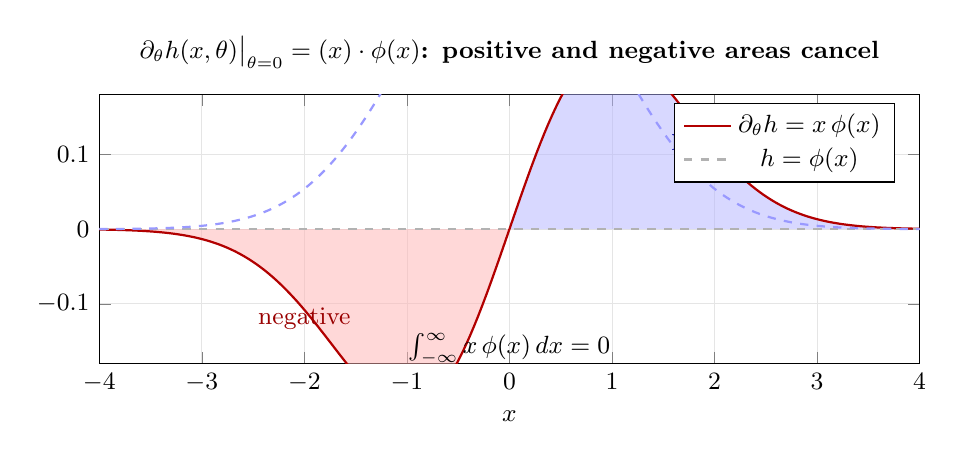
\begin{tikzpicture}
\begin{axis}[
  width=12cm, height=5cm,
  xlabel={$x$},
  title={$\partial_\theta h(x,\theta)\big|_{\theta=0}=(x)\cdot\phi(x)$: positive and negative areas cancel},
  xmin=-4, xmax=4, ymin=-0.18, ymax=0.18,
  domain=-4:4, samples=200,
  grid=both, grid style={line width=0.3pt, draw=gray!20},
  tick label style={font=\small},
  title style={font=\small\bfseries},
  label style={font=\small},
  legend pos=north east,
  legend style={font=\small},
]
% derivative of N(0,1) density w.r.t. theta = x * phi(x)
\addplot[thick, red!70!black, name path=curve] {x * exp(-x^2/2)/sqrt(2*3.14159)};
\addplot[name path=zero, draw=none] {0};
\addplot[red!30, opacity=0.5] fill between[of=curve and zero, soft clip={domain=-4:0}];
\addplot[blue!30, opacity=0.5] fill between[of=curve and zero, soft clip={domain=0:4}];
\addplot[thick, gray!60, dashed] {0};
\addplot[thick, blue!40, dashed, domain=-4:4, samples=200] {exp(-x^2/2)/sqrt(2*3.14159)};
\legend{$\partial_\theta h = x\,\phi(x)$, , , , $h=\phi(x)$}
\node[font=\small, red!60!black] at (axis cs:-2, -0.12) {negative};
\node[font=\small, blue!60!black] at (axis cs:2, 0.12) {positive};
\node[font=\small] at (axis cs:0, -0.16) {$\int_{-\infty}^{\infty} x\,\phi(x)\,dx = 0$};
\end{axis}
\end{tikzpicture}
\end{center}

The shaded areas are equal in magnitude.  This is Property~3 in
geometric form: the net signed area under $\partial_\theta h$ is zero.
This fact, on its own, has consequences --- but those will be drawn out
in Chapter~\ref{sec:score_fisher_chapter}, once we have introduced the
score.

%--------------------------------------------------------------------
\subsection{Pre-likelihood vs.\ likelihood: numeric vs.\ random argument}
\label{sec:prelikelihood}
%--------------------------------------------------------------------

So far the surface $h$ and its properties have involved no data: $h$
is a fixed bivariate function and all of its slices are deterministic
curves.  Once we acknowledge that observations are random, the same
surface gives rise to two different objects depending on what we plug
into its first slot --- a number, or a random variable.  This is the
distinction the Probabilist insists on, and it sets up everything in the next
two chapters: the random nature of the log-likelihood
(Chapter~\ref{sec:loglikelihood_chapter}), and the zero-mean property
of the score (Chapter~\ref{sec:score_fisher_chapter}).
%--------------------------------------------------------------------

So far we have treated $x$ as a deterministic argument --- a coordinate
along an axis.  Once we acknowledge that the observation is, formally,
a random variable $X:\Omega\to\mathbb{R}$, two different objects split
apart.  The Probabilist's terminology, which we follow here, draws the line by
\emph{what is plugged into the first slot of $h$}.

\paragraph{Pre-likelihood: first slot is a number.}
Fix a \emph{number} $x \in \mathbb{R}$, i.e.\ a point on the axis,
with no probabilistic structure attached.  The slice of $h$ at this
point is
\[
  L_x : \Theta \to \mathbb{R},
  \qquad
  L_x(\theta) \;:=\; h(x,\theta) \;=\; f_\theta(x).
\]
This is a deterministic function of $\theta$, indexed by a real
number $x$.  The Probabilist calls it the \textbf{pre-likelihood}.  The graph
of $L_x$ in the $(\theta, h)$ plane is a single, non-random curve.

\paragraph{Likelihood: first slot is a random variable.}
Now replace the number $x$ by $X(\omega)$ --- the random variable
itself, evaluated at a sample point $\omega \in \Omega$.  The result
is a function of two arguments:
\[
  L : \Omega \times \Theta \to \mathbb{R},
  \qquad
  L(\omega, \theta) \;:=\; f_\theta\bigl(X(\omega)\bigr)
  \;=\; L_{X(\omega)}(\theta).
\]
The Probabilist calls this the \textbf{likelihood} (proper).  Indexed by
$\omega$, it is a \emph{random} function of $\theta$: each draw of
$\omega$ gives a different curve $\theta \mapsto L(\omega,\theta)$.

\paragraph{What ``pre'' means here.}
The prefix \emph{pre} refers to ``before substituting the random
variable'', not to ``before taking the logarithm or maximising''.
Once we plug in the random observation, the object jumps from
deterministic to random:
\[
  \underbrace{L_x(\theta)}_{\text{indexed by number } x}
  \;\xrightarrow{\;x \,\leftarrow\, X(\omega)\;}\;
  \underbrace{L(\omega,\theta) \,=\, L_{X(\omega)}(\theta).}_{\text{indexed by } \omega}
\]
The map $\omega \mapsto L_{X(\omega)}$ is a random element of the
function space of curves $\Theta \to \mathbb{R}$.

\begin{remark}[A personal note]
This precise distinction is the Probabilist's preferred terminology and we adopt
it throughout the chapter.  Many textbooks call $L_x$ itself ``the
likelihood'' without making the $\omega$ vs.\ $x$ split explicit;
the present notation makes the measurability and randomness questions
that follow much cleaner to state.
\end{remark}

\paragraph{Key difference from the density.}
The density $f_\theta(x)$ integrates to $1$ over $x$ for every fixed
$\theta$ (this is Property~1 of $h$).  The pre-likelihood
$L_x(\theta)$ need \emph{not} integrate to $1$ over $\theta$;
it is not a density in $\theta$.  In the Bayesian framework one
multiplies $L_x$ by a prior $\pi(\theta)$ to obtain a proper
posterior density, but frequentist theory makes no such requirement.

\paragraph{Graphical reading of $L_x(\theta)$.}
For $\mathcal{N}(\theta, \sigma^2)$ the pre-likelihood at the
\emph{number} $x$ is
\[
  L_x(\theta) = \frac{1}{\sqrt{2\pi\sigma^2}}\exp\!\left(-\frac{(x-\theta)^2}{2\sigma^2}\right).
\]
As a function of $\theta$, this is bell-shaped, symmetric around
$\theta = x$, and maximised at $\hat\theta(x) = x$.  The plot below
draws three such pre-likelihood curves at three different
\emph{numeric} values of $x$.  When we later swap a number $x$ for
the random $X(\omega)$, each $\omega$ picks out one such curve
(determined by where on the axis $X(\omega)$ happens to land).

\begin{center}
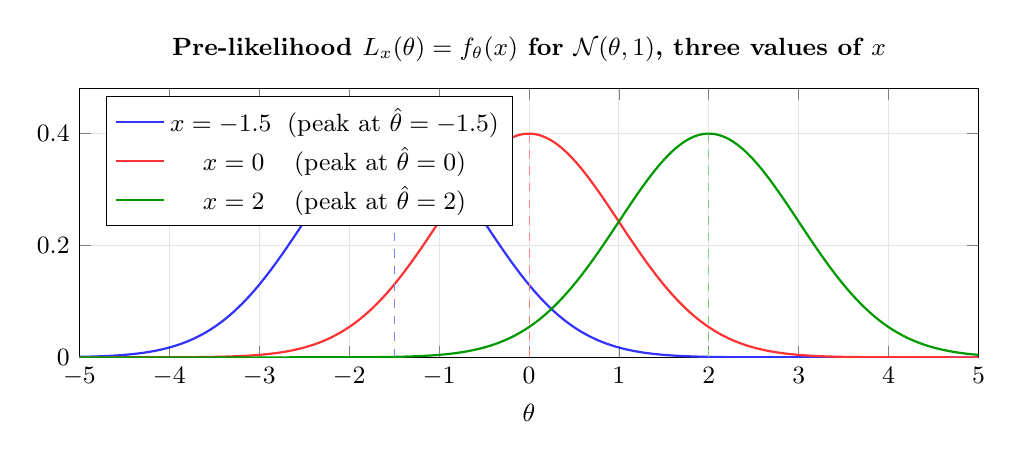
\begin{tikzpicture}
\begin{axis}[
  width=13cm, height=5cm,
  xlabel={$\theta$},
  title={Pre-likelihood $L_x(\theta)=f_\theta(x)$ for $\mathcal{N}(\theta,1)$, three values of $x$},
  xmin=-5, xmax=5, ymin=0, ymax=0.48,
  domain=-5:5, samples=200,
  grid=both, grid style={line width=0.3pt, draw=gray!20},
  tick label style={font=\small},
  title style={font=\small\bfseries},
  label style={font=\small},
  legend pos=north west, legend style={font=\small},
]
\addplot[thick, blue!80] {exp(-(x-(-1.5))^2/2)/sqrt(2*3.14159)};
\addplot[thick, red!80]  {exp(-(x-0)^2/2)/sqrt(2*3.14159)};
\addplot[thick, green!60!black] {exp(-(x-2)^2/2)/sqrt(2*3.14159)};
\addplot[dashed,blue!50,very thin] coordinates {(-1.5,0)(-1.5,0.399)};
\addplot[dashed,red!50,very thin] coordinates {(0,0)(0,0.399)};
\addplot[dashed,green!60!black!50,very thin] coordinates {(2,0)(2,0.399)};
\legend{$x=-1.5$\; (peak at $\hat\theta=-1.5$),
        $x=0$\;\;\; (peak at $\hat\theta=0$),
        $x=2$\;\;\; (peak at $\hat\theta=2$)}
\end{axis}
\end{tikzpicture}
\end{center}

Each curve peaks at the corresponding $x$ (since the MLE for
$\mathcal{N}(\theta,1)$ is $\hat\theta(x)=x$), but the shape ---
the curvature, the width --- is the same.  The curvature of
$L_x(\theta)$ at the MLE is $-1/\sigma^2$, which is the
(negative) Fisher information.

\paragraph{What the derivative of $L_{x_1}$ looks like.}
A small foreshadowing of Chapter~\ref{sec:score_fisher_chapter}: if
we differentiate the pre-likelihood $L_{x_1}(\theta)$ in $\theta$,
we get an odd S-shape.  Concretely, for $\mathcal{N}(\theta,1)$ at
$x_1 = 0$,
\[
  \frac{d L_{x_1}}{d\theta}
  \;=\; \frac{d}{d\theta}\,\varphi(x_1-\theta)
  \;=\; (x_1-\theta)\,\varphi(x_1-\theta)
  \;=\; -\theta\,\varphi(-\theta),
\]
an odd function of $\theta$ around $x_1$, with extrema at $\theta =
x_1 \pm 1$.  The Probabilist's hand-drawn picture below shows the shape.

\begin{figure}[H]
\centering
\includegraphics[width=0.7\textwidth]{fig_g_score_hand.png}
\caption{The derivative of the pre-likelihood, $\partial_\theta L_{x_1}(\theta)$,
for $\mathcal{N}(\theta,1)$ at $x_1 = 0$.  The Probabilist's label $L_{x_1}(\theta)$
on the figure refers to the slice itself; what is drawn is its
$\theta$-derivative.  The function is odd around $\theta = x_1$
with extrema at $\theta = x_1 \pm 1$, crosses zero at the MLE
$\hat\theta = x_1$, and integrates to zero over $\theta$
(by symmetry, just as the pre-likelihood does).  This curve
will reappear in Chapter~\ref{sec:score_fisher_chapter} as a
$\theta$-slice of the pre-score $s(x,\theta)$ at fixed $x = x_1$.}
\label{fig:g_score_hand}
\end{figure}

\paragraph{Not invariant under reparameterisation.}
The pre-likelihood is a function of $\theta$, so its shape depends
on how we parameterise the family.  If $\phi = q(\theta)$ is a
smooth bijection, the family $\{f_\theta\}$ can equally well be
written as $\{\tilde f_\phi\}$ with $\tilde f_\phi := f_{q^{-1}(\phi)}$,
and the pre-likelihood in the new parameter is
\[
  \tilde L_x(\phi) \;:=\; \tilde f_\phi(x) \;=\; f_{q^{-1}(\phi)}(x)
  \;=\; L_x\bigl(q^{-1}(\phi)\bigr).
\]
The \emph{values} are preserved at corresponding points: the height
of $\tilde L_x$ at $\phi$ equals the height of $L_x$ at
$\theta = q^{-1}(\phi)$.  In particular the MLE is preserved as a
point:
$\hat\phi(x) = q(\hat\theta(x))$.  But the \emph{shape} ---
concavity, curvature, width --- is generally \emph{not} preserved
unless $q$ is affine.  Reparameterising stretches and bends the
horizontal axis non-uniformly, so a strictly concave $L_x$ may become
non-concave in $\phi$, and the curvature at the MLE changes by the
factor $(q'(\hat\theta))^{-2}$.

A small concrete example: for $\mathcal{N}(\theta, 1)$ the pre-likelihood
$L_x(\theta)$ is a Gaussian bell in $\theta$ (strictly log-concave).
Reparameterise by $\phi = \theta^3$ (smooth bijection).  Then
$\tilde L_x(\phi) = L_x(\phi^{1/3})$, which is no longer log-concave
in $\phi$ near the origin: the cube-root rescaling flattens the curve
on one side of zero and steepens it on the other.  Same family, same
data, same inferential content; different shape.

This caveat is structural --- it has nothing to do with logs.  We
flag it now so that it does not have to be re-derived for the
log-likelihood in Chapter~\ref{sec:loglikelihood_chapter}.

\paragraph{From pre-likelihood to likelihood: randomising the index.}
Each curve in the plot above corresponds to a fixed number $x$.
The (proper) likelihood arises when, instead of choosing a particular
$x$, we let nature choose: $\omega \in \Omega$ is drawn, and we
look at the curve $L_{X(\omega)}$.  The likelihood is therefore a
\emph{random curve}.  Quantities computed from the likelihood
(the score, its variance, the Fisher information) are then naturally
random variables or expectations over $\omega$.

\paragraph{The pre-likelihood does not integrate to 1 over $\theta$.}
For the location-normal family the symmetry of the bell happens to
make $\int L_x(\theta)\,d\theta = 1$, but this is a coincidence:
the integral is a density in $\theta$ \emph{only because} the
density is a density in $x$ and the two coordinates are coupled
through $x-\theta$ alone.

A cleaner illustration uses the exponential model.  With
$f_\theta(x) = \theta e^{-\theta x}$ on $x>0$, $\theta>0$, the
pre-likelihood at the fixed number $x$ is
$L_x(\theta) = \theta e^{-\theta x}$ on $\theta>0$.  Its integral
over $\theta$ is
\[
  \int_0^\infty L_x(\theta)\,d\theta
  \;=\; \int_0^\infty \theta\,e^{-\theta x}\,d\theta
  \;=\; \frac{1}{x^2},
\]
which equals $1$ only at $x=1$ and depends on $x$ for every other
observation.  Normalisation of $L_x$ in $\theta$ is therefore not a
structural property; in this family it generically fails.

\begin{center}
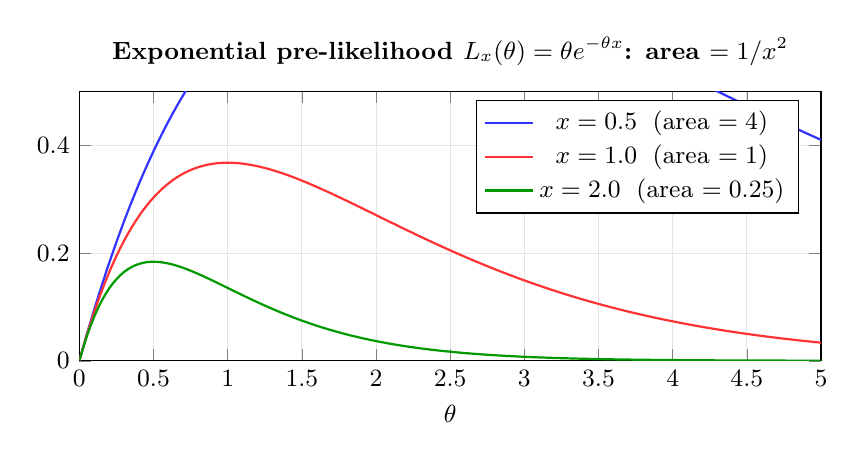
\begin{tikzpicture}
\begin{axis}[
  width=11cm, height=5cm,
  xlabel={$\theta$},
  title={Exponential pre-likelihood $L_x(\theta)=\theta e^{-\theta x}$: area $=1/x^2$},
  xmin=0, xmax=5, ymin=0, ymax=0.5,
  domain=0.001:5, samples=200,
  grid=both, grid style={line width=0.3pt, draw=gray!20},
  tick label style={font=\small},
  title style={font=\small\bfseries},
  label style={font=\small},
  legend pos=north east, legend style={font=\small},
]
\addplot[thick, blue!80]  {x*exp(-x*0.5)};
\addplot[thick, red!80]   {x*exp(-x*1.0)};
\addplot[thick, green!60!black] {x*exp(-x*2.0)};
\legend{$x=0.5$\; (area $=4$),
        $x=1.0$\; (area $=1$),
        $x=2.0$\; (area $=0.25$)}
\end{axis}
\end{tikzpicture}
\end{center}

The three curves all have peak at $\hat\theta(x) = 1/x$ but different
total areas: the pre-likelihood ``stretches'' or ``shrinks'' along
$\theta$ depending on the observed $x$, and the area under the curve
generally is not $1$.

%--------------------------------------------------------------------
\section{The Log-Likelihood}
\label{sec:loglikelihood_chapter}
%--------------------------------------------------------------------

Before we differentiate the likelihood to obtain the score, it is
worth pausing on the log transform itself.  Every property of the
log-likelihood that we will need --- additivity for i.i.d.\ samples,
preservation of the maximiser, concavity for exponential families ---
is a property of the function $\log L$ as a function of $\theta$,
\emph{before} any derivatives are taken.  Treating these properties
separately, in their own chapter, prevents them from being
silently absorbed into the score derivation.

%--------------------------------------------------------------------
\subsection{Why the logarithm}
%--------------------------------------------------------------------

The (pre-)likelihood is a product of densities and is typically very
small in absolute terms; it can underflow even modest sample sizes.
The log transform fixes several practical and structural
inconveniences at once.

\paragraph{Numeric reason: products become sums.}
For an i.i.d.\ sample $x_1,\ldots,x_n$ with density $f_\theta$,
the joint pre-likelihood at the numeric tuple $\mathbf{x}$ is
\[
  g_{\mathbf{x}}(\theta) \;=\; \prod_{i=1}^n f_\theta(x_i).
\]
A product of $n$ numbers, each of order $10^{-1}$ to $10^{-3}$,
underflows quickly.  The log:
\[
  \ell_{\mathbf{x}}(\theta) \;:=\; \log g_{\mathbf{x}}(\theta)
  \;=\; \sum_{i=1}^n \log f_\theta(x_i).
\]
A sum of well-behaved numbers, no underflow.

\paragraph{Structural reason: additivity.}
The log transform turns the product structure of i.i.d.\ likelihoods
into an additive one.  This is more than a numerical convenience: it
means that asymptotic theory (CLT, LLN) applies to the log-likelihood
directly --- to its first derivative the score
$\sum \partial_\theta \log f_\theta(x_i)$, and to its second derivative
the observed information $-\sum \partial^2_\theta \log f_\theta(x_i)$.
Without the log we would be working with products, where CLT-like
results require multiplicative analogues that are far less clean.

\paragraph{Geometric reason: products of bell curves are still bells.}
For the location-normal family, $f_\theta(x) = (2\pi)^{-1/2}
\exp\!\bigl(-(x-\theta)^2/2\bigr)$.  The pre-likelihood is
$\exp$ of a quadratic, so the log-likelihood is itself a quadratic
in $\theta$:
\[
  \ell_x(\theta) \;=\; -\tfrac{1}{2}\log(2\pi) - \tfrac{1}{2}(x-\theta)^2.
\]
A parabola, opening downward, with vertex at $\theta = x$.  We will
see in a moment that downward-parabolic log-likelihoods are
characteristic of a broad class (exponential families with quadratic
sufficient statistic), not just the normal.

%--------------------------------------------------------------------
\subsection{Definition and basic identities}
%--------------------------------------------------------------------

\paragraph{Pre-log-likelihood (numeric index).}
For a fixed number $x \in \mathbb{R}$, let
\[
  \Theta_x \;:=\; \{\theta \in \Theta : f_\theta(x) > 0\}
\]
be the set of parameter values for which $x$ has positive density.
Define
\[
  \ell_x: \Theta_x \to \mathbb{R},
  \qquad
  \ell_x(\theta) \;:=\; \log L_x(\theta) \;=\; \log f_\theta(x).
\]
This is a deliberate departure from the textbook convention of
extending $\log f_\theta(x)$ to all of $\Theta$ by setting it equal
to $-\infty$ on the zero-density set.  Per the Probabilist's recommendation,
we restrict the domain instead: $\ell_x$ lives on the positivity
set $\Theta_x$, takes real values only, and the symbol $-\infty$
never enters our formulas.

The motivation is integration.  Quantities like $\E_\theta[\ell_X]$
and $\E_\theta[(\partial_\theta \ell_X)^2]$ (the Fisher information)
are integrals of $\log$-of-density against the density itself.  When
$\log$ is allowed to take the value $-\infty$, every such integral
inherits a $0 \cdot \infty$ ambiguity that has to be resolved by
hand, conventions, or measure-theoretic gymnastics ($0 \cdot \infty
:= 0$ being the standard but easily-forgotten patch).  Restricting
the domain to $\Theta_x$ from the outset eliminates the ambiguity:
we never write $\log 0$, and every integral is over a region where
the integrand is finite and the density is positive.

\begin{remark}[When $\Theta_x$ depends on $x$]
For families with parameter-independent support (Gaussian, Poisson,
exponential families in canonical form), $\Theta_x = \Theta$ for
every $x$ in the support, and the restriction is vacuous.  The
restriction bites for families with $\theta$-dependent support such
as Uniform$[0,\theta]$: there, $\Theta_x = (x,\infty)$ for $x>0$,
and pre-log-likelihood is defined only for $\theta$ strictly larger
than the observed value.  This is precisely the family where the
regularity conditions for the score identity fail
(Remark in Section~\ref{sec:score_identity_derivation}); restricting
the domain makes the failure transparent rather than swept under a
$-\infty$ rug.
\end{remark}

\paragraph{The i.i.d.\ case and why we restrict to it.}
For an i.i.d.\ tuple $\mathbf{x} = (x_1,\ldots,x_n)$ the joint
positivity set is the intersection,
\[
  \Theta_{\mathbf{x}} \;=\; \bigcap_{i=1}^n \Theta_{x_i},
\]
and the joint pre-log-likelihood factors additively:
\[
  \ell_{\mathbf{x}}(\theta) \;=\; \sum_{i=1}^n \ell_{x_i}(\theta),
  \qquad \theta \in \Theta_{\mathbf{x}}.
\]
Both expressions rely heavily on the i.i.d.\ assumption.  Two things
are happening, and it is worth pulling them apart.

\emph{First}, the joint density factorises:
\[
  f_\theta^{(n)}(x_1,\ldots,x_n) \;=\; \prod_{i=1}^n f_\theta(x_i).
\]
This is why the log turns into a sum.

\emph{Second}, and more fundamentally, a single scalar parameter
$\theta$ suffices to describe the distribution of the entire random
vector $\mathbf{X} = (X_1,\ldots,X_n)$.  In the i.i.d.\ setting,
$\theta$ parameterises the common marginal $X_i \sim f_\theta$, and
the joint distribution is fully determined by $\theta$ together
with the independence assumption.  No additional parameters are
needed to specify the dependence structure --- there isn't any.

If we drop i.i.d., both of these break.  Suppose
$(X_1,\ldots,X_n)$ has an arbitrary joint distribution.  Then a
single $\theta$ governing the marginal of each $X_i$ is no longer
enough to characterise the joint distribution of $\mathbf{X}$: we
also need to specify the dependence between the $X_i$'s.  In
general, we need a richer parameter
$\boldsymbol{\eta}$ (typically vector-valued, sometimes
infinite-dimensional) indexing a family of joint densities
$\{f_{\boldsymbol{\eta}}^{(n)}\}$ on $\mathbb{R}^n$, and the
pre-log-likelihood becomes
\[
  \ell_{\mathbf{x}}(\boldsymbol{\eta})
  \;=\; \log f_{\boldsymbol{\eta}}^{(n)}(x_1,\ldots,x_n),
\]
which does \emph{not} decompose into a sum in any useful way.  Two
representative non-i.i.d.\ cases give a sense of where the difficulty
lies:

\begin{itemize}
\item \textbf{Identically distributed but dependent} (e.g.\ a
  stationary time series $\{X_t\}$).  Each $X_t$ has the same
  marginal $f_\theta$, but the joint density depends on
  $\theta$ \emph{and} on autocorrelation/copula parameters.  The
  marginal $\theta$ alone is not a sufficient parameterisation of
  $\mathbf{X}$.

\item \textbf{Independent but not identically distributed}
  (e.g.\ regression with non-random $X$, $Y_i \sim
  \mathcal{N}(\beta_0 + \beta_1 x_i, \sigma^2)$).  The joint
  density factorises, $f^{(n)} = \prod_i f_{\theta_i}$, but each
  marginal has its own parameter $\theta_i = \beta_0 + \beta_1 x_i$.
  The right object is the vector $\boldsymbol{\eta} =
  (\beta_0,\beta_1,\sigma^2)$, not a single $\theta$.
\end{itemize}

In both cases the log-likelihood is well-defined, but
$\theta$ alone is the wrong index.  Working out the score and
Fisher information for non-i.i.d.\ models requires care:
the additive structure of the i.i.d.\ score breaks, asymptotic
theory needs CLTs adapted to the dependence (mixing conditions,
martingale CLT) or to the heterogeneity (Lindeberg conditions),
and the information matrix may fail to be block-diagonal in ways
that complicate inversion.

\textbf{We do not pursue the non-i.i.d.\ direction in this text.}
From here on, the sample is i.i.d.\ unless stated otherwise, and
$\theta$ is a scalar parameter of the common marginal.  The
flagging above is meant only to say: this is a real boundary, and
the clean identities of the next two chapters live on the
i.i.d.\ side of it.

\paragraph{Log-likelihood (random index).}
Substituting $X_i(\omega)$ for the numeric tuple gives the
\textbf{log-likelihood}:
\[
  \mathcal{L}(\omega,\theta)
  \;:=\; \log L(\omega,\theta)
  \;=\; \sum_{i=1}^n \log f_\theta\bigl(X_i(\omega)\bigr),
  \qquad
  \theta \in \Theta_{X(\omega)},
\]
where $\Theta_{X(\omega)} = \bigcap_i \Theta_{X_i(\omega)}$ is now
itself random (a random subset of $\Theta$).  This is a random
function of $\theta$.  Each $\omega$ produces one realised
log-likelihood curve, defined on its own positivity slice.

\paragraph{Monotone equivalence with the likelihood.}
Since $\log$ is strictly increasing on $(0,\infty)$, the maximiser of
$\ell_x$ over $\Theta_x$ equals the maximiser of $L_x$ over the same
set:
\[
  \arg\max_{\theta\in\Theta_x} L_x(\theta)
  \;=\;
  \arg\max_{\theta\in\Theta_x} \ell_x(\theta).
\]
And since $L_x(\theta) = 0$ off $\Theta_x$, restricting the
argmax to $\Theta_x$ loses no maxima: any $\theta$ with
$L_x(\theta) = 0$ is dominated by points where $L_x > 0$.  So MLE
theory is universally formulated in terms of the log-likelihood:
nothing is lost by passing to logs, and additivity is gained.

%--------------------------------------------------------------------
\subsection{Concavity and exponential families}
%--------------------------------------------------------------------

\paragraph{Quadratic log-likelihood for the location-normal family.}
We saw above that for $\mathcal{N}(\theta,1)$,
$\ell_x(\theta) = -\tfrac12(x-\theta)^2 + \text{const}$ ---
a downward parabola.  For an i.i.d.\ sample this becomes
\[
  \ell_{\mathbf{x}}(\theta)
  \;=\; -\tfrac{1}{2}\sum_{i=1}^n (x_i-\theta)^2 + \text{const},
\]
still a downward parabola in $\theta$, with vertex at the sample mean
$\bar x = \frac{1}{n}\sum x_i$.  Concavity is uniform in $\mathbf{x}$,
and the maximiser is unique.

\paragraph{General exponential families: concavity in the natural parameter.}
A one-parameter exponential family in canonical form has density
\[
  f_\theta(x) \;=\; h_0(x) \exp\!\bigl(\theta\,T(x) - A(\theta)\bigr),
\]
where $T$ is the sufficient statistic and $A(\theta)$ is the
log-partition function.  Then
\[
  \ell_x(\theta) \;=\; \log h_0(x) + \theta\,T(x) - A(\theta).
\]
A fundamental result of exponential-family theory is that $A$ is
\emph{convex}; therefore $\ell_x$ is \emph{concave} in $\theta$
(strictly, when the family is minimal and identifiable).  Concavity
of the log-likelihood implies that any stationary point is a global
maximum, and gradient-based optimisation is well-posed.  This is the
deep reason that MLE in exponential families is computationally tame.

\paragraph{Non-concavity outside exponential families.}
Concavity is a property of exponential families, not of likelihoods
in general.  Mixture models, hidden-state models, and many
non-identifiable models have multimodal log-likelihoods.  This is
where EM and other iterative schemes earn their keep.

%--------------------------------------------------------------------
\subsection{The log-likelihood surface and its slices}
%--------------------------------------------------------------------

In direct analogy with $h(x,\theta) = f_\theta(x)$, define
\[
  \tilde h(x,\theta) \;:=\; \log f_\theta(x),
  \qquad
  (x,\theta) \in D, \;\; D := \{(x,\theta): f_\theta(x) > 0\}.
\]
The domain $D \subset \mathbb{R}\times\Theta$ is the positivity set
of the family --- the same region on which all our log-likelihood
slices live.  Outside $D$, $\tilde h$ is undefined; we do not assign
it the value $-\infty$.  This is the surface that the log-likelihood
and pre-log-likelihood slice up.  The two relevant directions:

\begin{itemize}
\item \textbf{Fixed $\theta$, varying $x$:}
  $\tilde h(\,\cdot\,,\theta_0)$ on the $\theta_0$-slice of $D$ is the
  log-density.  It does \emph{not} integrate to $1$ over $x$; instead,
  $\int e^{\tilde h}\,dx = 1$ (the integral being over the positivity
  slice, where the integrand $f_{\theta_0}$ is automatically zero
  off-slice anyway).  Differential entropy is
  $-\E_{\theta_0}[\tilde h(X,\theta_0)] = -\int_{\{f_{\theta_0}>0\}}
  f_{\theta_0} \log f_{\theta_0}\,dx$.

\item \textbf{Fixed $x$, varying $\theta$:}
  $\tilde h(x_1,\,\cdot\,)|_{\Theta_{x_1}} = \ell_{x_1}$ is the
  pre-log-likelihood, the workhorse of all that follows.
\end{itemize}

\begin{center}
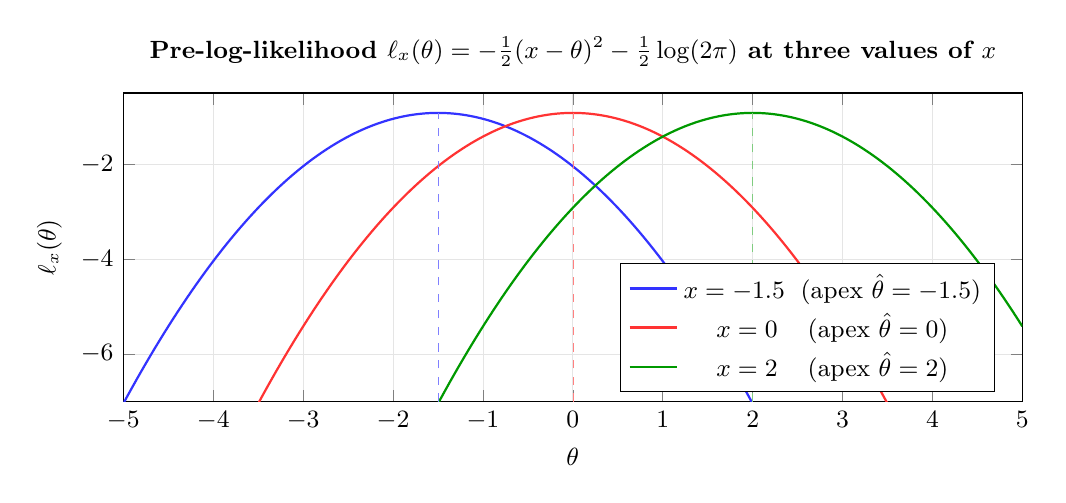
\begin{tikzpicture}
\begin{axis}[
  width=13cm, height=5.5cm,
  xlabel={$\theta$}, ylabel={$\ell_x(\theta)$},
  title={Pre-log-likelihood $\ell_x(\theta)=-\tfrac{1}{2}(x-\theta)^2 - \tfrac{1}{2}\log(2\pi)$ at three values of $x$},
  xmin=-5, xmax=5, ymin=-7, ymax=-0.5,
  domain=-5:5, samples=200,
  grid=both, grid style={line width=0.3pt, draw=gray!20},
  tick label style={font=\small},
  title style={font=\small\bfseries},
  label style={font=\small},
  legend pos=south east, legend style={font=\small},
]
\addplot[thick, blue!80] {-(x-(-1.5))^2/2 - 0.919};
\addplot[thick, red!80]  {-(x-0)^2/2 - 0.919};
\addplot[thick, green!60!black] {-(x-2)^2/2 - 0.919};
\addplot[dashed,blue!50,very thin] coordinates {(-1.5,-7)(-1.5,-0.919)};
\addplot[dashed,red!50,very thin] coordinates {(0,-7)(0,-0.919)};
\addplot[dashed,green!60!black!50,very thin] coordinates {(2,-7)(2,-0.919)};
\legend{$x=-1.5$\; (apex $\hat\theta=-1.5$),
        $x=0$\;\;\; (apex $\hat\theta=0$),
        $x=2$\;\;\; (apex $\hat\theta=2$)}
\end{axis}
\end{tikzpicture}
\end{center}

Compare to the pre-likelihood plot of
Section~\ref{sec:prelikelihood}: same peak locations, but the curves
are now strict parabolas opening downward.  The information about
where the apex sits is preserved; what changes is the shape further
from the apex --- parabolic decay (log-scale) vs.\ Gaussian decay
(linear scale).

%--------------------------------------------------------------------
\subsection{What the log-likelihood does not tell us}
%--------------------------------------------------------------------

A few honest caveats before we differentiate.  The log-likelihood is
the central object of frequentist inference, but it has its limits:

\begin{itemize}
\item \textbf{Not invariant under reparameterisation.}
  Like the (pre-)likelihood itself --- see the discussion in
  Section~\ref{sec:prelikelihood} --- the log-likelihood is not
  invariant under smooth reparameterisations $\phi = q(\theta)$:
  values match at corresponding points, but shape (concavity,
  curvature) is generally not preserved unless $q$ is affine.
  Taking the log does not save us here.

\item \textbf{Not directly a posterior log-density.}
  In Bayesian inference one adds $\log \pi(\theta)$ (the log prior)
  to obtain the log posterior, up to a normalising constant.  The
  log-likelihood by itself is not interpretable as a log-density in
  $\theta$.

\item \textbf{Comparable up to additive constants.}
  $\ell_x(\theta) + C$ contains the same inferential information as
  $\ell_x(\theta)$; only relative log-likelihoods matter.  This is
  why log-likelihood plots are often shown with the maximum
  subtracted, plotting $\ell_x(\theta) - \ell_x(\hat\theta)$.
\end{itemize}

We now have the structural setup to take derivatives.  In the next
chapter, $\partial_\theta \ell$ is the score, and
$-\partial_\theta^2 \ell$ the observed information --- objects
\emph{built from} the log-likelihood, not replacements for it.

%--------------------------------------------------------------------
\section{Score, Fisher Information, and the Information Identity}
\label{sec:score_fisher_chapter}
%--------------------------------------------------------------------

We now differentiate $\ell$ with respect to $\theta$.  The first
derivative is the score; the negative second derivative (in
expectation) is the Fisher information.  Before listing the score's
other properties, we cash in on the work done in Chapter 7: Property~3
(the vanishing $\theta$-integral of $\partial_\theta h$) was waiting
to deliver the zero-mean identity of the score, and now we collect.

\subsection{The density surface and what is differentiated}

We will work with the same surface $h(x,\theta) = f_\theta(x)$ ---
not because it is new, but because it is the right substrate.  The
score is the $\theta$-derivative of the log of this surface,
restricted to the data slice:
\[
  s(\theta) \;:=\; \partial_\theta \ell_x(\theta)
  \;=\; \frac{\partial_\theta h(x,\theta)}{h(x,\theta)}
  \;=\; \partial_\theta \log f_\theta(x).
\]
The score is a function of $\theta$ indexed by $x$ (pre-score) or by
$\omega$ (score proper, after substituting $X(\omega)$).

%--------------------------------------------------------------------
\subsection{The semi-elasticity operator: algebra before semantics}
\label{sec:semi_elasticity_operator}
%--------------------------------------------------------------------

The score is one instance of a single differential operator applied
to a positive function.  Before specialising to likelihoods, it is
worth collecting the operator's general properties --- they explain
several features of the score (additivity for i.i.d.\ samples,
behaviour under reparameterisation, Fisher information identity) at
the algebraic level, without any probability.

\paragraph{Definition.}
Let $\mathcal{P}$ be the set of positive, differentiable real-valued
functions on an open set $U \subset \mathbb{R}$.  The
\textbf{semi-elasticity operator} is the map
\[
  D: \mathcal{P} \longrightarrow F(U),
  \qquad
  D[f](t) \;:=\; \frac{f'(t)}{f(t)} \;=\; (\log f)'(t),
\]
where $F(U)$ is just ``the set of real-valued functions on $U$'' ---
\emph{not} necessarily continuous ones.  The point is subtle and is
worth being explicit about.

\begin{remark}[Why we cannot write $D: \mathcal{P} \to C(U)$]
\label{rem:derivative_not_continuous}
A function $f$ being differentiable on $U$ does not imply that its
derivative $f'$ is continuous on $U$.  The classical counterexample
is
\[
  f(t) \;=\;
  \begin{cases}
    t^2 \sin(1/t), & t \neq 0,\\
    0, & t = 0,
  \end{cases}
\]
defined on all of $\mathbb{R}$.  This $f$ is differentiable
everywhere (one checks $f'(0)=0$ directly from the limit definition),
but
\[
  f'(t) \;=\; 2t\sin(1/t) - \cos(1/t)
  \qquad (t\neq 0),
\]
which oscillates between roughly $-1$ and $+1$ as $t\to 0$ and has no
limit at $0$.  So $f \in \mathcal{P}$ (after shifting upward to keep
it positive) does not imply $D[f] \in C(U)$.

Such examples are pathological --- they are constructed on purpose
and do not arise from any parametric family we care about --- but
they show that the codomain ``$C(U)$'' I wrote earlier is technically
wrong.  If we want a clean operator with continuous output, we have
to restrict the source: let $\mathcal{P}_1 \subset \mathcal{P}$ be
the set of positive $C^1$ functions on $U$.  Then
\[
  D: \mathcal{P}_1 \longrightarrow C(U)
\]
is genuinely continuous-valued, because $f \in \mathcal{P}_1$ has
$f'\in C(U)$, $1/f \in C(U)$ (since $f>0$ continuous), and the
product $f'/f$ is then in $C(U)$.

For everything we do with likelihoods of standard parametric
families, the underlying densities are $C^\infty$ in $\theta$, so
the pre-log-likelihoods live in $\mathcal{P}_1$ (in fact in $C^\infty$),
and the codomain question never bites.  We retain the wider domain
$\mathcal{P}$ for generality but acknowledge that $D[f]$ is then a
``mere'' function, not automatically a continuous one.
\end{remark}

Two reformulations:
\[
  D[f] \;=\; \frac{f'}{f} \;=\; (\log f)'.
\]
The first is the algebraic ratio of $f'$ and $f$; the second is the
derivative of $\log f$.  These are the two genuinely distinct ways
of writing $D$; the choice of notation for the derivative ($f'$
vs.\ $df/dt$ vs.\ $\partial_t f$) is immaterial.  Because $f$ has
just one (scalar) argument $t$, the appropriate symbol is the
\emph{total} derivative $d/dt$; we use $f'$ throughout for brevity,
reserving $\partial_t$ for the partial derivative in $\theta$ later,
once the second argument $x$ enters the picture.
The semi-elasticity name comes from definition~(iii) of
Section~\ref{sec:score_elasticity}.

\paragraph{$D$ as a composition: two paths through intermediate spaces.}
The two reformulations above correspond to two different
\emph{factorisations} of $D$ through more elementary operators.  Set
up the relevant function spaces first:
\begin{align*}
  \mathcal{P}_1 &:= \{f: U\to\mathbb{R} \;:\; f>0,\; f\in C^1\}
   \qquad \text{(positive, } C^1 \text{)}\\
  C(U) &:= \text{continuous real-valued functions on } U\\
  C^1(U) &:= \text{continuously differentiable functions on } U
\end{align*}
(We restrict to $\mathcal{P}_1$ in this diagram so the codomain of
$D$ is genuinely $C(U)$; see Remark~\ref{rem:derivative_not_continuous}
for what happens on the wider class $\mathcal{P}$.)

The three elementary operators we will compose are:
\begin{align*}
  \log&: \mathcal{P}_1 \to C^1(U), & f &\mapsto \log f \qquad
    \text{(pointwise: zeroth-order local)}\\
  d/dt&: C^1(U) \to C(U), & g &\mapsto g'  \qquad
    \text{(neighbourhood: first-order local)}\\
  \div&: C^1(U) \to C(U), & f' &\mapsto f'/f
    \qquad \text{(pointwise, with $f\in\mathcal{P}_1$ fixed)}
\end{align*}

Both paths from $\mathcal{P}_1$ to $C(U)$ give the same answer:
\[
\begin{tikzcd}[row sep=large, column sep=huge]
  & C^1(U) \arrow[dr, "d/dt"] & \\
  \mathcal{P}_1 \arrow[ur, "\log"] \arrow[dr, "d/dt"', swap] \arrow[rr, "D", dashed] & & C(U) \\
  & C^1(U) \arrow[ur, "\,\div f"', swap] &
\end{tikzcd}
\]

\textbf{Path A (upper):}
$\;f \;\xrightarrow{\;\log\;}\; \log f \;\xrightarrow{\;d/dt\;}\; (\log f)'.$
First take the log pointwise; then differentiate.

\textbf{Path B (lower):}
$\;f \;\xrightarrow{\;d/dt\;}\; f' \;\xrightarrow{\;\div f\;}\; f'/f.$
First differentiate; then divide pointwise by $f$ (which we still
have available, since we are tracking $f$ alongside the computation
of $f'$).

Equality of the two paths is the chain rule applied to $\log$:
\[
  (\log f)'(t) \;=\; \frac{1}{f(t)}\cdot f'(t) \;=\; \frac{f'(t)}{f(t)}.
\]

The two paths are equal as operators, but they have different
rhetorical force.  Path A says ``differentiate the log-likelihood''
--- the standard textbook framing.  Path B says ``divide the gradient
by the value'' --- the framing that makes clear why constants kill
($D[c\cdot f] = D[f]$) and why the score respects multiplication.
In computations we will freely move between them.

\paragraph{Intermediate spaces have different ``geographies''.}
A subtle point worth flagging: the two intermediate spaces in the
diagram are both copies of $C^1(U)$, but they are reached by quite
different maps from $\mathcal{P}_1$.

Path A takes the log first, going from $\mathcal{P}_1$ (positive
functions) into a copy of $C^1(U)$ that may contain unbounded
negative values (since $\log f \to -\infty$ as $f \to 0^+$).  The
positivity of $f$ is no longer visible; only the absence of zero
values is preserved (as $\log f$ being finite).

Path B differentiates first, going into a copy of $C^1(U)$ that can
contain negative values too (since $f'$ can be negative wherever $f$
is decreasing).  The positivity of $f$ is preserved, but only
implicitly, as the fact that we are still allowed to divide by it
in the next step.

The two intermediate routes pass through different ``regions'' of
function space, but converge to the same answer.

\paragraph{The two paths have different domains.}
A sharper version of the previous point: viewed as abstract operators
on a class of functions, Paths A and B are not defined on the same
class.

\textbf{Path B} ($d/dt$ then $\div f$) is defined wherever $f$ is
\emph{differentiable and non-vanishing}.  The output $f'/f$ is a
formal semi-elasticity, available even for functions that take
negative values (e.g.\ $f(t) = -e^{-t}$ gives $f'/f = -1$).

\textbf{Path A} ($\log$ then $d/dt$) is defined only where $f$ is
\emph{differentiable and strictly positive}, since $\log$ requires
positivity.  On a function that takes negative values, Path A fails
at the first step.

So Path B has a wider natural domain than Path A.  On the
intersection --- positive differentiable $f$ --- the two paths agree
and the diagram of the previous paragraph commutes.  But the
``semi-elasticity'' $f'/f$ as a bare ratio exists for a larger class
of $f$ than the log-derivative interpretation does.

For likelihood theory this distinction is moot: densities are
non-negative, and on their positivity set they are strictly positive,
so both paths apply.  But when the same operator appears outside
the likelihood context --- for instance in growth-rate calculations
in economics, where the underlying quantity may be negative ---
only Path B remains a meaningful definition.

\paragraph{Locality.}
A key feature of $D$ that we will use without comment is that it is
a \emph{local} operator: $D[f](t_0)$ depends only on $f$ in an
arbitrarily small neighbourhood of $t_0$.  More precisely, each
constituent step of Paths A and B is local in a sharp sense:

\begin{itemize}
\item \textbf{Pointwise (zeroth-order locality).}
  The map $f \mapsto \log f$ is even more local than ``local'':
  $\log f(t_0)$ depends only on $f$ at the single point $t_0$, not on
  a neighbourhood.  It is a pointwise transformation.  The same is
  true of division by $f$, multiplication by a function, and any
  composition of $f$ with a fixed real-valued function $g$, giving
  $g\circ f$.

\item \textbf{Neighbourhood (first-order locality).}
  Differentiation $f \mapsto f'$ requires more than a single value:
  $f'(t_0)$ is defined as a limit of difference quotients
  $(f(t_0+h)-f(t_0))/h$, so we need $f$ on a small interval
  containing $t_0$.  But the interval can be arbitrarily small.
  Second-order locality means: any modification of $f$ \emph{outside}
  a neighbourhood of $t_0$, however large, leaves $f'(t_0)$
  unchanged.
\end{itemize}

The composite $D = (d/dt) \circ \log$ inherits the weaker of the
two: $D[f](t_0)$ requires $f$ on a neighbourhood (first-order local).

This contrasts sharply with the \emph{integral} operators that will
appear when we take expectations.  The map
\[
  f \;\longmapsto\; \E_\theta[f]
  \;=\; \int f(x)\,p(x\mid\theta)\,dx
\]
is \emph{global}: its value at $\theta$ depends on $f$ over the entire
data axis.  Changing $f$ on any region of positive measure changes
the integral.  This is why differentiating before integrating
(Property 3 of Chapter~\ref{sec:density_and_likelihood}: $\int
\partial_\theta h\,dx = 0$) is non-trivial: it interchanges a local
operator $\partial_\theta$ with a global operator $\int dx$, and the
interchange needs the regularity conditions we keep citing.  The
score identity $\E_\theta[s] = 0$ is, structurally, an identity
relating the action of one local operator ($D$) and one global
operator ($\E_\theta$) on the same surface $h$.

\paragraph{Domain.}
$D[f]$ is well-defined wherever $f > 0$ and $f$ is differentiable.
Positivity matters: $\log f$ has to make sense, and the ratio $f'/f$
fails to be continuous (or even defined) where $f$ vanishes.  This
is the operator-level reason for restricting the domain to the
positivity set $\Theta_x$ when defining the pre-log-likelihood
(Section~\ref{sec:prelikelihood}): outside $\Theta_x$, $D$ is not
applicable.

For non-smooth $f$ (e.g.\ Laplace density, which has a kink at $\mu$),
$D[f]$ is undefined at the kink and one needs subgradients or
distributional derivatives; we set such cases aside.

\paragraph{Property 1: Not additive --- multiplicative.}
The operator $D$ is \emph{not} a linear / additive operator on
$\mathcal{P}$.  Adding two positive functions in general gives a
new positive function, but
\[
  D[f+g] \;=\; \frac{f' + g'}{f + g}
  \;\neq\; D[f] + D[g]
\]
in general.  No clean formula for the sum exists.  This is the
reason we never write a score for ``the likelihood plus a constant''
or for mixture models in closed form.

What $D$ \emph{does} respect is \textbf{multiplication}:
\[
  D[fg] \;=\; \frac{(fg)'}{fg} \;=\; \frac{f'g + fg'}{fg}
  \;=\; \frac{f'}{f} + \frac{g'}{g} \;=\; D[f] + D[g].
\]
Multiplication of $f$'s becomes addition of $D[f]$'s.  Equivalently:
\[
  D[fg] = D[f] + D[g],
  \qquad
  D[f/g] = D[f] - D[g],
  \qquad
  D[f^\alpha] = \alpha\,D[f] \;\; (\alpha\in\mathbb{R}).
\]
This is exactly why i.i.d.\ samples give additive scores: the joint
likelihood $L(\theta) = \prod_i f_\theta(x_i)$ is a product, and
$D = \partial_\theta\log$ converts that product into a sum
$s(\theta) = \sum_i \partial_\theta \log f_\theta(x_i)$.  The
additivity of the score is not an accident --- it is the operator
algebra of $D$ applied to a product.

\paragraph{Property 2: Iteration.}
Apply $D$ twice (with respect to the same variable):
\[
  D^2[f] \;=\; D\!\left[\frac{f'}{f}\right]
  \;=\; \frac{d}{dt}\!\left(\frac{f'}{f}\right)
  \;=\; \frac{f''}{f} - \left(\frac{f'}{f}\right)^2
  \;=\; \frac{f''}{f} - D[f]^2.
\]
So $D^2[f]$ does \emph{not} equal $f''/f$; there is a quadratic
correction.  Rearranging,
\[
  \frac{f''}{f} \;=\; D^2[f] + D[f]^2
  \;=\; (\log f)'' + \bigl((\log f)'\bigr)^2.
\]
This identity will reappear shortly as the \textbf{information
identity}: when $f$ is a likelihood, $-\E[D^2 \ell]$ (the expected
observed information) equals $\E[D[\ell]^2]$ (the variance of the
score), and the cross term $f''/f$ has zero expectation under the
true parameter --- a direct consequence of $\int \partial_\theta^2 h
\,dx = 0$, which is Property~3 differentiated again.

\paragraph{Property 3: Reparameterisation (chain rule).}
If $\phi = q(\theta)$ is a smooth bijection and $\tilde f(\phi) =
f(q^{-1}(\phi))$, then by the chain rule
\[
  D_\phi[\tilde f](\phi)
  \;=\; \frac{\tilde f'(\phi)}{\tilde f(\phi)}
  \;=\; \frac{f'(q^{-1}(\phi))\cdot (q^{-1})'(\phi)}{f(q^{-1}(\phi))}
  \;=\; (q^{-1})'(\phi) \cdot D_\theta[f]\bigl(q^{-1}(\phi)\bigr).
\]
The semi-elasticity transforms by the \emph{Jacobian} of the inverse
reparameterisation, not invariantly.  In particular, the score is
\emph{not} invariant under reparameterisation: $s_\phi(\phi) =
s_\theta(\theta)/q'(\theta)$.  This is the operator-level statement
of the caveat from Section~\ref{sec:prelikelihood}.

\paragraph{Property 4: Zero of $D[f]$ = stationary point of $\log f$ = stationary point of $f$.}
Since $D[f] = (\log f)'$ and $\log$ is strictly increasing,
$D[f](t_0) = 0 \iff (\log f)'(t_0) = 0 \iff f'(t_0) = 0$.  Zeros of
the semi-elasticity coincide with stationary points of the original
$f$.  Applied to the likelihood, this is the first-order condition
for the MLE: $s(\hat\theta) = 0 \iff L'(\hat\theta) = 0$.

\paragraph{Property 5: Non-injectivity and the fibres of $D$.}
$D$ is not injective: many different $f$'s give the same $D[f]$.
This is worth comparing to the ordinary derivative, since the
fibres look different in the two cases.

\textbf{Fibres of $d/dt$.}
If $g'_1 = g'_2$, then $g_1 - g_2$ has zero derivative, so
$g_1 - g_2 = c$ for some constant $c$.  The pre-image of any given
derivative is a family of \emph{parallel translates}:
\[
  (d/dt)^{-1}(g') \;=\; \{g + c : c \in \mathbb{R}\}.
\]
Vertical shifts are invisible to differentiation.

\textbf{Fibres of $D$.}
If $D[f_1] = D[f_2]$, then $(\log f_1)' = (\log f_2)'$, so
$\log f_1 - \log f_2 = $ const, i.e.\ $f_1 / f_2 = $ const.  The
pre-image is a family of \emph{positive proportions}:
\[
  D^{-1}(D[f]) \;=\; \{c \cdot f : c > 0\}.
\]
Multiplicative rescalings are invisible to $D$.

The parallel is clean: differentiation forgets additive constants,
the semi-elasticity operator forgets multiplicative ones.  This is
exactly the operator-level statement that likelihoods are defined
only up to a positive multiplicative constant --- the score (and
everything built from it: Fisher information, MLE, tests) depends
on the equivalence class $\{c \cdot L : c > 0\}$, not on the
particular representative.  Two likelihoods that differ by a
normalising constant give the same inference.

In compact form: $D$ factors through the quotient
$\mathcal{P}_1 / \!\sim$, where $f \sim g \iff f = cg$ for some
$c > 0$.

\paragraph{Summary table.}
\[
\begin{array}{l|l}
\text{Property of } D & \text{Consequence for the score}\\\hline
D[fg] = D[f] + D[g] & \text{i.i.d.\ scores are additive: } s = \sum_i s_i\\
D^2[f] = f''/f - D[f]^2 & \text{information identity (after expectation)}\\
D_\phi[\tilde f] = (q^{-1})'\cdot D_\theta[f] & \text{score not invariant under reparam.}\\
D[f](t_0)=0 \iff f'(t_0)=0 & \text{score MLE condition} = \text{likelihood MLE}\\
D^{-1}(D[f]) = \{cf : c>0\} & \text{score depends on shape, not scale}\\
\text{not additive: } D[f+g] \neq D[f]+D[g] & \text{mixtures have no closed-form score}\\
\end{array}
\]

\noindent The next subsection applies $D$ to the density to recover the
zero-mean property of the score.

%--------------------------------------------------------------------
\subsection{From Property~3 to the score identity}
\label{sec:score_identity_derivation}
%--------------------------------------------------------------------

Property~3 of Chapter~\ref{sec:density_and_likelihood} says
$\int \partial_\theta h\,dx = 0$.  Now divide and multiply by $h$
inside the integral (assuming $h>0$):
\[
  0 = \int_{\mathbb{R}} \frac{\partial h}{\partial\theta}\,dx
  = \int_{\mathbb{R}} \frac{\partial h/\partial\theta}{h(x,\theta)}\cdot h(x,\theta)\,dx
  = \int_{\mathbb{R}} \frac{\partial \log h}{\partial\theta}\cdot h(x,\theta)\,dx
  = \E_\theta\!\left[\frac{\partial \log f_\theta}{\partial\theta}\right]
  = \E_\theta[s(\theta)].
\]

So the score has zero mean \emph{under the true parameter} --- not by
coincidence, not as a separate axiom, but as a direct consequence of
the fact that the density integrates to one.  The derivation is a
chain:
\[
  \underbrace{\int h\,dx = 1}_{\text{density axiom}}
  \;\xrightarrow{\;\text{diff.\ w.r.t.\ }\theta\;}\;
  \underbrace{\int \partial_\theta h\,dx = 0}_{\text{Property 3}}
  \;\xrightarrow{\;\div h,\;\times h\;}\;
  \underbrace{\E_\theta[s] = 0.}_{\text{score identity}}
\]

\begin{remark}[What the regularity condition does]
The step ``differentiate under the integral'' requires justification
--- one needs to exchange $\frac{d}{d\theta}$ and $\int$.  Sufficient
conditions (dominated convergence) are satisfied for exponential
families, Gaussian models, and most textbook parametric models.  For
the Uniform$[0,\theta]$ family this interchange fails (the support
depends on $\theta$), and indeed $\E[s]\neq 0$.  The score is
$s=-n/\theta<0$ everywhere, which is consistent with the failure of
the zero-mean property.
\end{remark}

\paragraph{Graphical summary of the chain.}
The figure below shows the three steps as a sequence of panels.

\begin{center}
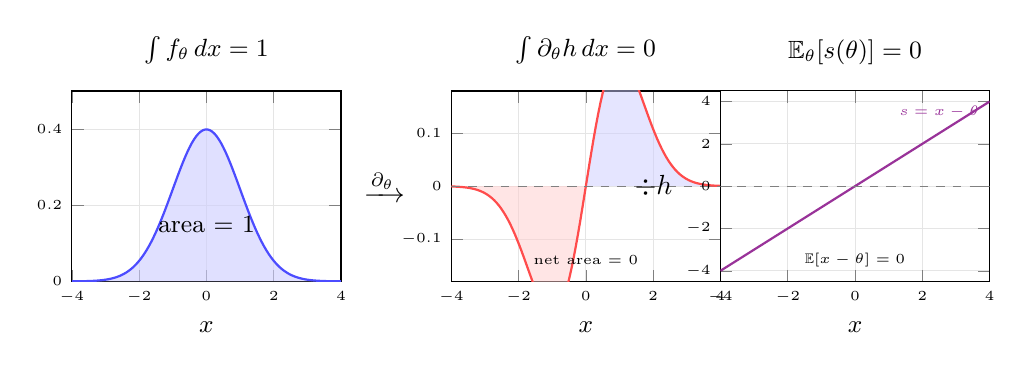
\begin{tikzpicture}
% Panel 1: density integrates to 1
\begin{axis}[
  name=p1,
  width=5cm, height=4cm,
  xlabel={$x$}, title={$\int f_\theta\,dx = 1$},
  xmin=-4,xmax=4,ymin=0,ymax=0.5,
  domain=-4:4, samples=120,
  grid=both, grid style={line width=0.3pt,draw=gray!20},
  tick label style={font=\tiny},
  title style={font=\small\bfseries},
  label style={font=\small},
]
\addplot[thick,blue!70,name path=f] {exp(-x^2/2)/sqrt(2*3.14159)};
\addplot[name path=zero,draw=none]{0};
\addplot[blue!20,opacity=0.6] fill between[of=f and zero];
\node[font=\small] at (axis cs:0,0.15) {area = 1};
\end{axis}
% arrow
\node at ($(p1.east)+(0.55cm,0)$) {$\xrightarrow{\partial_\theta}$};
% Panel 2: derivative integrates to 0
\begin{axis}[
  name=p2,
  at={(p1.east)}, anchor=west, xshift=1.4cm,
  width=5cm, height=4cm,
  xlabel={$x$}, title={$\int \partial_\theta h\,dx = 0$},
  xmin=-4,xmax=4,ymin=-0.18,ymax=0.18,
  domain=-4:4, samples=120,
  grid=both, grid style={line width=0.3pt,draw=gray!20},
  tick label style={font=\tiny},
  title style={font=\small\bfseries},
  label style={font=\small},
]
\addplot[thick,red!70,name path=d]{x*exp(-x^2/2)/sqrt(2*3.14159)};
\addplot[name path=zero2,draw=none]{0};
\addplot[red!20,opacity=0.5] fill between[of=d and zero2,soft clip={domain=-4:0}];
\addplot[blue!20,opacity=0.5] fill between[of=d and zero2,soft clip={domain=0:4}];
\addplot[dashed,gray]{0};
\node[font=\tiny] at (axis cs:0,-0.14) {net area = 0};
\end{axis}
% arrow
\node at ($(p2.east)+(0.55cm,0)$) {$\div h$};
% Panel 3: E[score] = 0
\begin{axis}[
  name=p3,
  at={(p2.east)}, anchor=west, xshift=1.4cm,
  width=5cm, height=4cm,
  xlabel={$x$}, title={$\E_\theta[s(\theta)]=0$},
  xmin=-4,xmax=4,ymin=-4.5,ymax=4.5,
  domain=-4:4, samples=120,
  grid=both, grid style={line width=0.3pt,draw=gray!20},
  tick label style={font=\tiny},
  title style={font=\small\bfseries},
  label style={font=\small},
]
\addplot[thick,violet!80]{x};
\addplot[dashed,gray]{0};
\node[font=\tiny,violet!80] at (axis cs:2.5,3.5) {$s=x-\theta$};
\node[font=\tiny] at (axis cs:0,-3.5) {$\E[x-\theta]=0$};
\end{axis}
\end{tikzpicture}
\end{center}

\begin{definition}
The \textbf{score} is the derivative of the log-likelihood with
respect to the parameter:
\[
  s(\theta) = \frac{\partial}{\partial\theta}\,\ell(\theta)
  = \frac{\partial}{\partial\theta}\log p(\mathbf{x}\mid\theta).
\]
For an i.i.d.\ sample:
$s(\theta) = \sum_{i=1}^n \frac{\partial}{\partial\theta}\log p(x_i\mid\theta)$.
\end{definition}

Two fundamental properties:

\textbf{(i) At the MLE, score is zero:}
$s(\hat\theta_\mathrm{MLE}) = 0$ --- the first-order condition for
an interior maximum (see Section~\ref{sec:nonsmooth} for exceptions).

\textbf{(ii) Under the true parameter, score has zero mean:}
$\E_\theta[s(\theta)] = 0$.
Proof: differentiate $\int p(x\mid\theta)\,dx = 1$ under the integral
sign, use $\partial_\theta\log p = \frac{1}{p}\partial_\theta p$.

\paragraph{Several parameters: the gradient.}
When $\theta\in\mathbb{R}^p$, the score is the gradient vector
$\mathbf{s}(\theta)=\nabla_\theta\ell(\theta)$; the MLE satisfies
$\mathbf{s}(\hat\theta)=\mathbf{0}$.

\subsection{Score as a semi-elasticity of the likelihood}
\label{sec:score_elasticity}

There are several notions of elasticity; they differ in which
argument is differentiated in absolute vs.\ relative (logarithmic)
terms.  Let $f(t)>0$ be a differentiable function.

\paragraph{Three definitions.}

\textbf{(i) Full (log-log) elasticity} --- relative change in $f$
per relative change in $t$:
\[
  \varepsilon^{\log\text{-}\log}(t)
  = \frac{d\log f}{d\log t}
  = t\cdot\frac{d\log f}{dt}
  = \frac{t}{f(t)}\cdot f'(t).
\]
Dimensionless.  Both $f$ and $t$ enter through logarithms.

\textbf{(ii) Semi-elasticity of $f$ with respect to $\log t$
(log-level)} --- absolute change in $f$ per relative change in $t$:
\[
  \varepsilon^{f\text{-}\log t}(t)
  = \frac{df}{d\log t}
  = t\cdot f'(t).
\]

\textbf{(iii) Semi-elasticity of $\log f$ with respect to $t$
(log-level, the other way)} --- relative change in $f$ per absolute
change in $t$:
\[
  \varepsilon^{\log f\text{-}t}(t)
  = \frac{d\log f}{dt}
  = \frac{f'(t)}{f(t)}.
\]
This takes the logarithm of $f$ only, not of $t$.

\paragraph{The score is definition (iii).}
Applying it to the likelihood $L(\theta)$:
\[
  \frac{d\log L}{d\theta}
  = \frac{L'(\theta)}{L(\theta)}
  = s(\theta).
\]
The score is the semi-elasticity of the likelihood $L$ with respect
to the parameter $\theta$: the proportional change in the likelihood
per unit absolute change in $\theta$.  It takes the logarithm of
$L$ but \emph{not} of $\theta$.

\begin{remark}[Relation to the full elasticity]
The full log-log elasticity of $L$ is
$\varepsilon^{\log\text{-}\log}(\theta)
 = \theta\cdot s(\theta)$.
This is \emph{not} the score; it differs by a factor of $\theta$.
At the MLE both vanish (since $s(\hat\theta)=0$ and $\hat\theta\neq 0$
generically), so they give the same optimality condition, but they
are different objects.
\end{remark}

\begin{figure}[h]
\centering
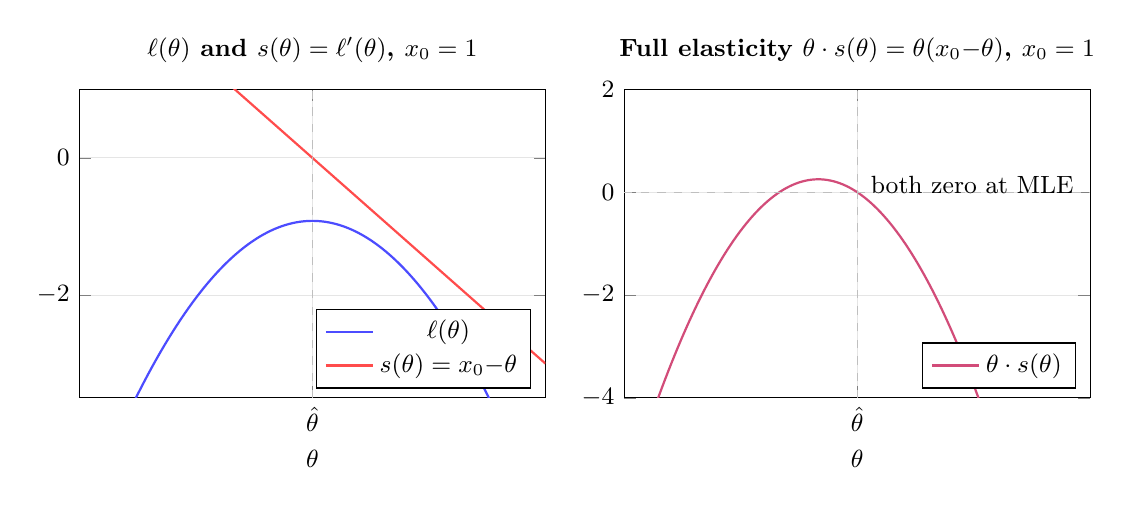
\begin{tikzpicture}
% Left panel: ell(theta) and score s(theta) for N(mu,1), x0=1
\begin{axis}[
  name=left,
  width=7.5cm, height=5.5cm,
  xlabel={$\theta$},
  title={$\ell(\theta)$ and $s(\theta)=\ell'(\theta)$, $x_0=1$},
  xmin=-2, xmax=4, ymin=-3.5, ymax=1,
  domain=-2:4, samples=150,
  grid=both, grid style={line width=0.3pt,draw=gray!20},
  tick label style={font=\small},
  title style={font=\small\bfseries},
  label style={font=\small},
  legend pos=south east, legend style={font=\small},
  xtick={1}, xticklabels={$\hat\theta$},
]
% log-likelihood: ell = -0.5*(x-theta)^2 - 0.5*log(2*pi), x0=1
\addplot[thick,blue!70]{-0.5*(1-x)^2 - 0.919};
% score: s = x0 - theta = 1 - theta
\addplot[thick,red!70]{1-x};
\addplot[dashed,gray!50] coordinates{(1,-3.5)(1,1)};
\legend{$\ell(\theta)$, $s(\theta)=x_0{-}\theta$}
\end{axis}
% Right panel: full log-log elasticity theta*s(theta)
\begin{axis}[
  at={($(left.east)+(1.0cm,0)$)}, anchor=west,
  width=7.5cm, height=5.5cm,
  xlabel={$\theta$},
  title={Full elasticity $\theta\cdot s(\theta)=\theta(x_0{-}\theta)$, $x_0=1$},
  xmin=-2, xmax=4, ymin=-4, ymax=2,
  domain=0.01:4, samples=150,
  grid=both, grid style={line width=0.3pt,draw=gray!20},
  tick label style={font=\small},
  title style={font=\small\bfseries},
  label style={font=\small},
  legend pos=south east, legend style={font=\small},
  xtick={1}, xticklabels={$\hat\theta$},
]
\addplot[thick,purple!70,domain=-2:4]{x*(1-x)};
\addplot[dashed,gray!50] coordinates{(1,-4)(1,2)};
\addplot[dashed,gray!50,domain=-2:4,samples=2]{0};
\node[font=\small,anchor=west] at (axis cs:1.05,0.15) {both zero at MLE};
\legend{$\theta\cdot s(\theta)$}
\end{axis}
\end{tikzpicture}
\caption{Left: log-likelihood $\ell(\theta)=\log L(\theta)$ and
  score $s(\theta)=\ell'(\theta)=d\log L/d\theta$ --- the
  semi-elasticity (definition iii).
  Right: full log-log elasticity $\theta\cdot s(\theta)
  =\partial\log L/\partial\log\theta$ (definition i).
  Both vanish at the MLE; they are different functions of $\theta$.}
\label{fig:elasticity}
\end{figure}

\subsection{Fisher information and the information identity}

For the normal model $\mathcal{N}(\mu,\sigma^2)$ the two Fisher
informations are:
\[
  \mathcal{I}_\mu = \frac{1}{\sigma^2},
  \qquad
  \mathcal{I}_{\sigma^2} = \frac{1}{2\sigma^4}.
\]
The information matrix (both parameters jointly) is diagonal:
\[
  \mathcal{I}(\mu,\sigma^2) =
  \begin{pmatrix} 1/\sigma^2 & 0 \\ 0 & 1/(2\sigma^4) \end{pmatrix}.
\]

\subsubsection{The three-way identity}

The Fisher information satisfies the following chain of equalities:
\[
  \mathcal{I}(\theta)
  \;=\; \Var_\theta[s(\theta)]
  \;=\; \E_\theta\!\left[s(\theta)^2\right]
  \;=\; -\E_\theta\!\left[\frac{\partial^2 \ell}{\partial\theta^2}\right].
\]

The first equality holds because $\E[s(\theta)]=0$ (under the true
parameter), so variance equals the second moment.
The third equality --- $\E[s^2] = -\E[\ell'']$ --- is the
\textbf{information equality} (Bartlett's second identity).

\subsubsection{Proof of the information equality (the Probabilist, $n=1$)}

We give the Probabilist's proof for $n=1$, which is slightly more detailed in
its intermediate steps than the streamlined version below.

\medskip
\noindent\textbf{Step 1: second derivative of a logarithm.}
Let $y=f(\theta)$ and $z=\ln y = \ln f(\theta)$.  Then
\[
  \frac{dz}{d\theta}
  = \frac{d}{d\theta}\ln f(\theta)
  = \frac{1}{f(\theta)}\cdot f'(\theta),
\]
and differentiating once more:
\[
  \frac{d^2z}{d\theta^2}
  = \frac{d}{d\theta}\!\left(\frac{f'(\theta)}{f(\theta)}\right)
  = \frac{f''(\theta)\cdot f(\theta) - (f'(\theta))^2}{(f(\theta))^2}
  = \frac{f''(\theta)}{f(\theta)} - \left(\frac{f'(\theta)}{f(\theta)}\right)^{\!2}.
\]
So for any positive differentiable $f$:
\[
  (\ln f)'' = \frac{f''}{f} - \left(\frac{f'}{f}\right)^{\!2}.
  \tag{$*$}
\]

\medskip
\noindent\textbf{Step 2: introduce the second variable $x$.}
Abusing notation slightly (using $f$ for what is usually written $p$
or $h$), set $f(x,\theta)$ a joint function and define
\[
  z(x,\theta) := \frac{\partial^2}{\partial\theta^2}\ln f(x,\theta)
  = \frac{\partial^2 f/\partial\theta^2}{f(x,\theta)}
    - \left(\frac{\partial f/\partial\theta}{f(x,\theta)}\right)^{\!2}.
\]

\medskip
\noindent\textbf{Step 3: substitute $x\mapsto X(\omega)$ and take
expectation.}
For an abstract probability measure $P$ on $\Omega$:
\[
  \E_P\bigl[z(X(\omega),\theta)\bigr]
  = \E_P\!\left[\frac{\partial^2 f/\partial\theta^2\,(X(\omega),\theta)}
                     {f(X(\omega),\theta)}\right]
  - \E_P\!\left[\left(\frac{\partial f/\partial\theta\,(X(\omega),\theta)}
                           {f(X(\omega),\theta)}\right)^{\!2}\,\right].
\]
Now suppose $P$ has density $p(x)$ (with respect to Lebesgue
measure). The expectations become integrals.  The second term on the
right is $\E_P[s^2]$ where $s(x,\theta)=\partial_\theta\ln f(x,\theta)$
is the score.  We focus on the \emph{minuend} (first term):
\[
  \text{minuend}
  = \E_P\!\left[\frac{\partial^2 f(x,\theta)/\partial\theta^2}
                     {f(x,\theta)}\right]
  = \int_{\mathbb{R}}
      \frac{\partial^2 f(x,\theta)/\partial\theta^2}{f(x,\theta)}
      \cdot p(x)\,dx.
\]
For a general $p$ we cannot simplify this further.

\medskip
\noindent\textbf{Step 4: specialise to $p(x)=f(x,\theta)$.}
Under the true model the sampling density equals $f(\cdot,\theta)$,
so $p(x)=f(x,\theta)$ and the minuend becomes
\[
  \text{minuend}\big|_{p=f}
  = \int_{\mathbb{R}}
      \frac{\partial^2 f(x,\theta)/\partial\theta^2}{f(x,\theta)}
      \cdot f(x,\theta)\,dx
  = \int_{\mathbb{R}} \frac{\partial^2 f(x,\theta)}{\partial\theta^2}\,dx.
\]
Under the regularity assumption that differentiation and integration
may be exchanged:
\[
  \text{minuend}\big|_{p=f}
  = \frac{\partial^2}{\partial\theta^2}\int_{\mathbb{R}} f(x,\theta)\,dx
  = \frac{\partial^2}{\partial\theta^2}\,1
  = \frac{\partial}{\partial\theta}\,0 = 0.
\]

\medskip
\noindent\textbf{Conclusion.}
With the minuend equal to zero, the identity $(*)$ under $\E[\,\cdot\,]$
gives
\[
  \E\bigl[z(X,\theta)\bigr]
  = 0 - \E\bigl[s^2(X,\theta)\bigr],
\]
i.e.\ $\E[z] = -\E[s^2]$.  Since $z=(\ln f)''=\ell''$ and
$s=(\ln f)'=\ell'$, this reads
\[
  \boxed{
    \mathcal{I}_{f(\cdot,\theta)}(\theta)
    = \E\bigl[s^2(X,\theta)\bigr]
    = -\E\!\left[\frac{\partial^2}{\partial\theta^2}\ell(X,\theta)\right].
  }
\]

\subsubsection{Proof of the information equality (streamlined)}

We know $\E_\theta[s(\theta)] = 0$ for all $\theta$, i.e.\
\[
  \int s(x,\theta)\,p(x\mid\theta)\,dx = 0 \quad \forall\,\theta.
\]
Differentiate both sides with respect to $\theta$:
\[
  \int \frac{\partial s}{\partial\theta}\,p\,dx
  + \int s\,\frac{\partial p}{\partial\theta}\,dx = 0.
\]
The first integral is $\E[\partial s/\partial\theta] = \E[\ell'']$.
For the second, note $\partial p/\partial\theta = p \cdot s$
(since $s = \partial\log p/\partial\theta$), so the second integral is
$\int s^2 p\,dx = \E[s^2]$.  Therefore:
\[
  \E[\ell''] + \E[s^2] = 0
  \;\implies\;
  \boxed{\E[s^2] = -\E[\ell''].}
\]

\subsubsection{Geometric interpretation}

The identity says: \emph{on average over the data, the square of the
slope of the log-likelihood equals minus the curvature of the
log-likelihood}.

\begin{itemize}
  \item $\ell''(\theta) < 0$ at a maximum (concave down): $-\E[\ell'']>0$ makes sense as a measure of information.
  \item Large curvature $|\ell''|$ (sharply peaked log-likelihood)
    means the score $s$ varies steeply with $\theta$, so data are
    highly informative about $\theta$.
  \item Small curvature (flat log-likelihood) means the score is
    nearly flat --- the likelihood barely responds to changes in
    $\theta$, so data are weakly informative.
\end{itemize}

\subsubsection{The pre-integral quantity: score squared}

A subtle but important point: $\mathcal{I}(\theta) = \E[s(\theta)^2]$
is a number --- an expectation.  The quantity \emph{under the integral}
is $s(x,\theta)^2$, a \textbf{random variable} (it depends on $x$).
This pre-integral object has no universally agreed name; one sometimes
sees it called the \emph{score contribution} or \emph{observed
information contribution}.

Its distribution is determined by the model: for
$\mathcal{N}(\mu,\sigma^2)$ with $n=1$,
\[
  s = \frac{x-\mu}{\sigma^2} \sim \mathcal{N}\!\left(0,\,\frac{1}{\sigma^2}\right),
  \qquad
  s^2 \sim \frac{1}{\sigma^2}\,\chi^2_1.
\]
The mean of $s^2$ equals $1/\sigma^2 = \mathcal{I}$ --- this is the
information equality by definition.  But the distribution of $s^2$ is
\emph{right-skewed} (chi-squared); the Fisher information is just its
expectation, not the full distribution.

\begin{figure}[h]
\centering
% 4-panel Fisher information identity figure
% sigma^2=1.5, mu_true=2, x_0=2 (single observation at true mean for illustration)
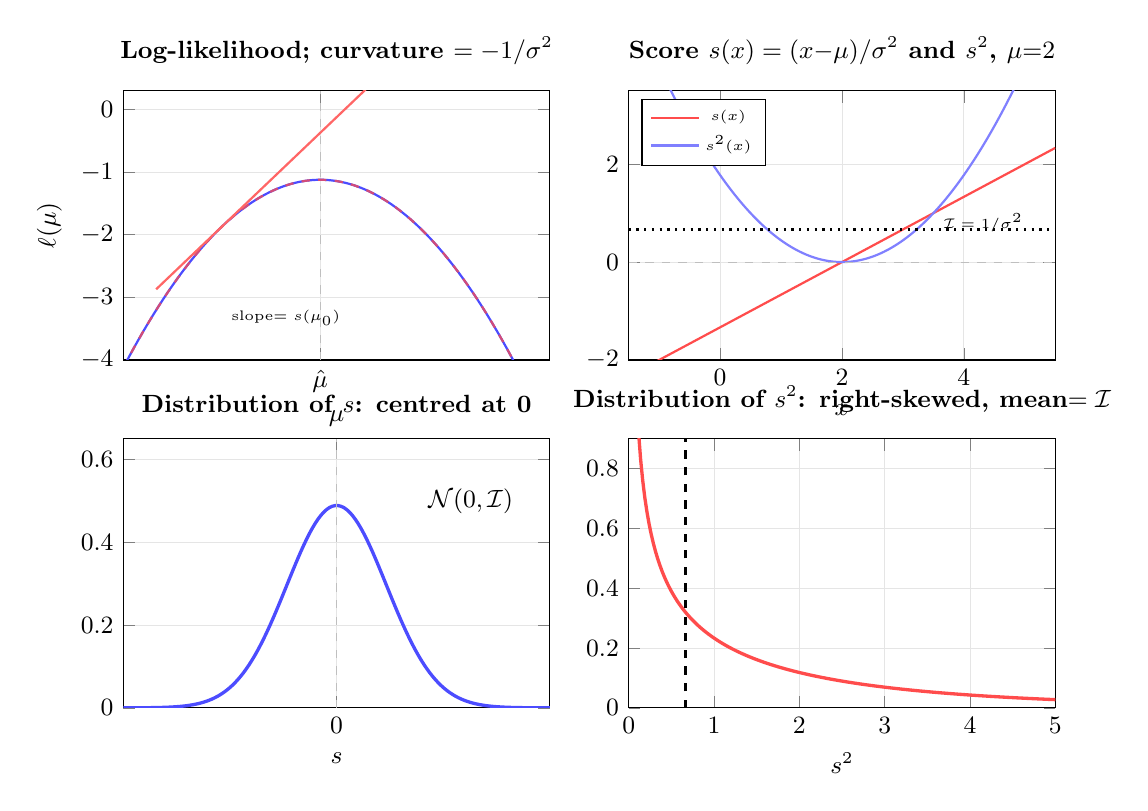
\begin{tikzpicture}
% Top-left: log-likelihood with curvature and tangent
\begin{axis}[
  name=tl,
  width=7cm, height=5cm,
  xlabel={$\mu$}, ylabel={$\ell(\mu)$},
  title={Log-likelihood; curvature $=-1/\sigma^2$},
  xmin=-1, xmax=5.5, ymin=-4, ymax=0.3,
  domain=-1:5.5, samples=150,
  grid=both, grid style={line width=0.3pt,draw=gray!20},
  tick label style={font=\small},
  title style={font=\small\bfseries,align=center},
  label style={font=\small},
  xtick={2}, xticklabels={$\hat\mu$},
]
% ell(mu|x0=2), sigma^2=1.5: -0.5*(2-mu)^2/1.5 - const
\addplot[thick,blue!70]{-0.5*(2-x)^2/1.5 - 0.5*ln(2*3.14159*1.5)};
% osculating parabola at mu=2 (same, shown dashed purple)
\addplot[thick,dashed,purple!70]{-0.5*(2-x)^2/1.5 - 0.5*ln(2*3.14159*1.5)};
% tangent at mu0=0.5: slope = s(x0=2, mu0=0.5) = (2-0.5)/1.5=1
\addplot[thick,red!60,domain=-0.5:3]{(-0.5*(2-0.5)^2/1.5 - 0.5*ln(2*3.14159*1.5)) + (2-0.5)/1.5*(x-0.5)};
\addplot[dashed,gray!50] coordinates{(2,-4)(2,0.3)};
\node[font=\tiny,anchor=south west] at (axis cs:0.5,-3.6)
  {slope$=s(\mu_0)$};
\end{axis}
% Top-right: score and score-squared as functions of x
\begin{axis}[
  name=tr,
  at={($(tl.east)+(1cm,0)$)}, anchor=west,
  width=7cm, height=5cm,
  xlabel={$x$},
  title={Score $s(x)=(x{-}\mu)/\sigma^2$ and $s^2$, $\mu{=}2$},
  xmin=-1.5, xmax=5.5, ymin=-2, ymax=3.5,
  domain=-1.5:5.5, samples=150,
  grid=both, grid style={line width=0.3pt,draw=gray!20},
  tick label style={font=\small},
  title style={font=\small\bfseries,align=center},
  label style={font=\small},
  legend pos=north west, legend style={font=\tiny},
]
% s(x,mu=2) = (x-2)/1.5
\addplot[thick,red!70]{(x-2)/1.5};
% s^2
\addplot[thick,blue!50]{((x-2)/1.5)^2};
% horizontal line at I = 1/sigma^2 = 1/1.5
\addplot[dotted,black,thick,domain=-1.5:5.5,samples=2]{1/1.5};
\addplot[dashed,gray!50,domain=-1.5:5.5,samples=2]{0};
\node[font=\tiny,anchor=west] at (axis cs:3.5,0.8)
  {$\mathcal{I}=1/\sigma^2$};
\legend{$s(x)$,$s^2(x)$}
\end{axis}
% Bottom-left: histogram of s (approximated by N(0,I) curve)
\begin{axis}[
  name=bl,
  at={($(tl.south)-(0,1cm)$)}, anchor=north,
  width=7cm, height=5cm,
  xlabel={$s$},
  title={Distribution of $s$: centred at 0},
  xmin=-3.5, xmax=3.5, ymin=0, ymax=0.65,
  domain=-3.5:3.5, samples=150,
  grid=both, grid style={line width=0.3pt,draw=gray!20},
  tick label style={font=\small},
  title style={font=\small\bfseries,align=center},
  label style={font=\small},
  xtick={0}, xticklabels={$0$},
]
% N(0, I) = N(0, 1/1.5): sd = sqrt(1.5) ~ 1.225
\addplot[very thick,blue!70]{exp(-x^2*1.5/2)/sqrt(2*3.14159/1.5)};
\addplot[dashed,gray!50] coordinates{(0,0)(0,0.65)};
\node[font=\small] at (axis cs:2.2,0.5) {$\mathcal{N}(0,\mathcal{I})$};
\end{axis}
% Bottom-right: distribution of s^2 ~ (1/sigma^2)*chi^2_1
\begin{axis}[
  name=br,
  at={($(tr.south)-(0,1cm)$)}, anchor=north,
  width=7cm, height=5cm,
  xlabel={$s^2$},
  title={Distribution of $s^2$: right-skewed, mean$=\mathcal{I}$},
  xmin=0, xmax=5, ymin=0, ymax=0.9,
  domain=0.01:5, samples=150,
  grid=both, grid style={line width=0.3pt,draw=gray!20},
  tick label style={font=\small},
  title style={font=\small\bfseries,align=center},
  label style={font=\small},
]
% (1/sigma^2)*chi^2_1 pdf = (sigma^2/(2)) * (1/sqrt(2*pi)) * (sigma^2*u)^{-1/2} * exp(-sigma^2*u/2)
% = 1/sqrt(2*pi*sigma^2*u) * exp(-u/(2*sigma^2)); sigma^2=1.5
\addplot[very thick,red!70,domain=0.04:5,samples=200]
  {1/sqrt(2*3.14159*1.5*x)*exp(-x/(2*1.5))};
% vertical dashed at mean = I = 1/1.5 ~ 0.667
\addplot[dashed,black,thick] coordinates{(0.667,0)(0.667,0.9)};
\node[font=\small,anchor=south] at (axis cs:0.667,0.9)
  {$\mathcal{I}$};
\end{axis}
\end{tikzpicture}
\caption{Four panels illustrating the information identity for
  $\mathcal{N}(\mu,\sigma^2)$ with $\sigma^2=1.5$, $\mu_\mathrm{true}=2$.
  Top-left: log-likelihood $\ell(\mu|x_1)$ with curvature
  $\ell_{\mu\mu}=-1/\sigma^2$ (osculating parabola, purple dashed)
  and a tangent at $\mu_0\neq\hat\mu$ whose slope is the score.
  Top-right: score $s(x,\mu_\mathrm{true})=(x-\mu)/\sigma^2$ and
  $s^2$ as functions of $x$; the horizontal dotted line marks
  $\mathcal{I}=E[s^2]=1/\sigma^2$.
  Bottom-left: $\mathcal{N}(0,\mathcal{I})$ density (limiting distribution of $s$);
  centred at 0.
  Bottom-right: $(1/\sigma^2)\chi^2_1$ density (distribution of $s^2$);
  right-skewed; its mean (dashed) equals $\mathcal{I}$.}
\label{fig:fisher_identity}
\end{figure}

Large $\mathcal{I}$: sharply curved log-likelihood, precise MLE.
Small $\mathcal{I}$: flat log-likelihood, imprecise MLE.

\begin{center}
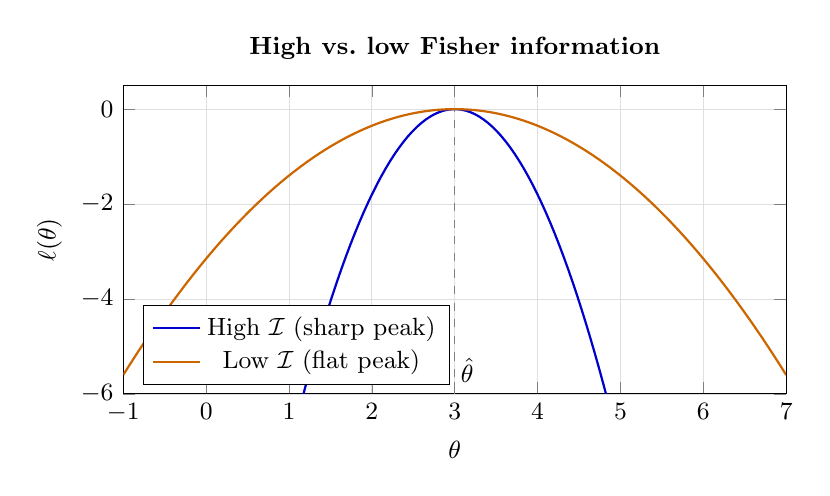
\begin{tikzpicture}
\begin{axis}[
  width=10cm, height=5.5cm,
  xlabel={$\theta$}, ylabel={$\ell(\theta)$},
  title={High vs.\ low Fisher information},
  grid=both, grid style={line width=0.3pt, draw=gray!25},
  xmin=-1, xmax=7, ymin=-6, ymax=0.5,
  domain=-1:7, samples=150,
  legend pos=south west, legend style={font=\small},
  tick label style={font=\small},
  title style={font=\small\bfseries},
  label style={font=\small}
]
\addplot[thick, blue!80!black]  {-1.8*(x-3)^2};
\addplot[thick, orange!80!black]{-0.35*(x-3)^2};
\legend{High $\mathcal{I}$ (sharp peak), Low $\mathcal{I}$ (flat peak)}
\draw[dashed,gray] (axis cs:3,-6) -- (axis cs:3,0);
\node[font=\small] at (axis cs:3.15,-5.5) {$\hat\theta$};
\end{axis}
\end{tikzpicture}
\end{center}

\begin{figure}[h]
\centering
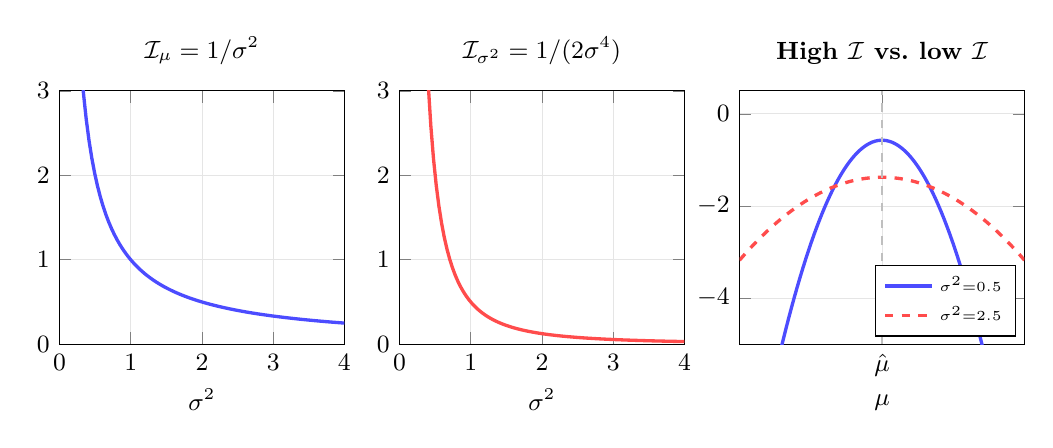
\begin{tikzpicture}
% Left: I_mu = 1/sigma^2 as function of sigma^2
\begin{axis}[
  name=left,
  width=5.2cm, height=4.8cm,
  xlabel={$\sigma^2$},
  title={$\mathcal{I}_\mu=1/\sigma^2$},
  xmin=0, xmax=4, ymin=0, ymax=3,
  domain=0.1:4, samples=100,
  grid=both, grid style={line width=0.3pt,draw=gray!20},
  tick label style={font=\small},
  title style={font=\small\bfseries},
  label style={font=\small},
]
\addplot[very thick,blue!70]{1/x};
\end{axis}
% Centre: I_sigma^2 = 1/(2*sigma^4)
\begin{axis}[
  name=centre,
  at={($(left.east)+(0.7cm,0)$)}, anchor=west,
  width=5.2cm, height=4.8cm,
  xlabel={$\sigma^2$},
  title={$\mathcal{I}_{\sigma^2}=1/(2\sigma^4)$},
  xmin=0, xmax=4, ymin=0, ymax=3,
  domain=0.25:4, samples=100,
  grid=both, grid style={line width=0.3pt,draw=gray!20},
  tick label style={font=\small},
  title style={font=\small\bfseries},
  label style={font=\small},
]
\addplot[very thick,red!70]{1/(2*x^2)};
\end{axis}
% Right: sharp vs flat log-likelihood
\begin{axis}[
  at={($(centre.east)+(0.7cm,0)$)}, anchor=west,
  width=5.2cm, height=4.8cm,
  xlabel={$\mu$},
  title={High $\mathcal{I}$ vs.\ low $\mathcal{I}$},
  xmin=-2, xmax=4, ymin=-5, ymax=0.5,
  domain=-2:4, samples=100,
  grid=both, grid style={line width=0.3pt,draw=gray!20},
  tick label style={font=\small},
  title style={font=\small\bfseries},
  label style={font=\small},
  legend pos=south east, legend style={font=\tiny},
  xtick={1}, xticklabels={$\hat\mu$},
]
% high I: sigma^2=0.5
\addplot[very thick,blue!70]{-0.5*(1-x)^2/0.5 - 0.5*ln(2*3.14159*0.5)};
% low I: sigma^2=2.5
\addplot[very thick,red!70,dashed]{-0.5*(1-x)^2/2.5 - 0.5*ln(2*3.14159*2.5)};
\addplot[dashed,gray!50] coordinates{(1,-5)(1,0.5)};
\legend{$\sigma^2{=}0.5$, $\sigma^2{=}2.5$}
\end{axis}
\end{tikzpicture}
\caption{Fisher information for the normal model.
  Left: $\mathcal{I}_\mu=1/\sigma^2$ as a function of $\sigma^2$.
  Centre: $\mathcal{I}_{\sigma^2}=1/(2\sigma^4)$ --- faster decay;
  estimating variance is harder than estimating mean for large $\sigma$.
  Right: sharp (high $\mathcal{I}$) vs.\ flat (low $\mathcal{I}$)
  log-likelihood; same MLE $\hat\mu=x_1$.}
\label{fig:fisher_info}
\end{figure}

%--------------------------------------------------------------------
\subsection{Score properties: a compact reference}
\label{sec:score_reference}
%--------------------------------------------------------------------

\subsubsection{Two distinct zeros}

The score $s(x,\theta)$ is a function of \emph{two} arguments and
appears in two different zero conditions that are often confused.

\textbf{Zero mean under the true parameter} (a property of the
distribution):
\[
  \E_{\theta_0}\!\left[s(\,\cdot\,,\theta_0)\right] = 0.
\]
Here $x$ is random (drawn from $p(\cdot|\theta_0)$) and
$\theta_0$ is fixed.  Both the sampling measure and the argument of
$s$ use the \emph{same} $\theta_0$.  Short version:
\emph{measure and score argument coincide.}

\textbf{Zero at the MLE} (a property of a specific dataset):
\[
  s(x_{\mathrm{obs}},\,\hat\theta) = 0.
\]
Here $x_{\mathrm{obs}}$ is fixed (the observed sample) and $\theta$
varies.  This is the first-order optimality condition; it requires
$\ell$ to be differentiable and $\hat\theta$ to be in the interior
of $\Theta$ (see Section~\ref{sec:nonsmooth}).

\textbf{What breaks centring.}
If the sampling measure is $P_{\theta_0}$ but the score is evaluated
at a different $\theta_1 \neq \theta_0$:
\[
  \E_{\theta_0}\!\left[s(\,\cdot\,,\theta_1)\right] \neq 0
  \quad \text{in general.}
\]
The measure and the argument diverge; centring fails.  This is
exactly the situation under the alternative hypothesis $H_1$.

\subsubsection{LLN and CLT for the score (the Probabilist)}

\noindent\textbf{Score for a sample is a sum.}
For $n=1$, the score is
\[
  s(x,\theta) = \frac{\partial_\theta f_\theta(x)}{f_\theta(x)}.
\]
For an i.i.d.\ sample $(x_1,\ldots,x_n)$ the joint density is
$f_\theta(x_1)\cdots f_\theta(x_n)$, and by the product rule for $D$
(Property~1 of Section~3.2):
\[
  s(x_1,\ldots,x_n;\theta)
  = \frac{\partial_\theta[f_\theta(x_1)\cdots f_\theta(x_n)]}
         {f_\theta(x_1)\cdots f_\theta(x_n)}
  = \frac{\partial_\theta f_\theta(x_1)}{f_\theta(x_1)}
    + \cdots +
    \frac{\partial_\theta f_\theta(x_n)}{f_\theta(x_n)}
  = s(\theta,x_1) + \cdots + s(\theta,x_n).
\]
Denoting $Y_i(\omega) := s(\theta, X_i(\omega))$: having i.i.d.\ $X_i$
we get i.i.d.\ $Y_i$ with zero mean (score identity), and
\[
  s(X_1,\ldots,X_n;\theta) = Y_1 + \cdots + Y_n,
  \qquad
  \E\,s(X_1,\ldots,X_n;\theta) = 0.
\]

\medskip
\noindent\textbf{LLN: $n$ is too much.}
Dividing by $n$:
\[
  \tfrac{1}{n}\,s(X_1,\ldots,X_n;\theta)
  = \bar Y_n
  \;\xrightarrow{\;\mathrm{a.s.}\;}\; \E Y_1 = 0.
\]
Norming by $n$ makes the score degenerate to zero.

\medskip
\noindent\textbf{CLT: divide by $\sqrt{n}$.}
\[
  \frac{1}{\sqrt{n}}\,s(X_1,\ldots,X_n;\theta)
  \;\xrightarrow{d}\; \mathcal{N}(0,\sigma^2),
  \quad \sigma^2 = \Var Y_1. \tag{1}
\]
By the information identity, that variance equals the Fisher information:
\[
  \mathcal{I}(\theta) = \Var\,s(\theta,X_1) = \Var Y_1.
\]
Normalising to a standard pivot:
\[
  \frac{1}{\sqrt{n}\,\sqrt{\Var\,s(X_1;\theta)}}
  \bigl(s(X_1;\theta)+\cdots+s(X_n;\theta)\bigr)
  \;\xrightarrow{d}\; \mathcal{N}(0,1). \tag{2}
\]

\medskip
\noindent\textbf{CLT for squares: $\chi^2$ limit.}
From the base CLT~(2), convergence for squares:
\[
  \frac{1}{n\,\mathcal{I}_1(\theta)}\,
  s^2(X_1,\ldots,X_n;\theta)
  \;\xrightarrow{d}\; \chi^2_1. \tag{3}
\]
Note $n\cdot\mathcal{I}_1(\theta)=\mathcal{I}_n(\theta)$, so (3) can
be written
\[
  \frac{s^2(X_1,\ldots,X_n;\theta)}{\mathcal{I}_n(\theta)}
  \;\xrightarrow{d}\; \chi^2_1.
\]

\subsubsection{The square of the CLT: diagonal and off-diagonal decomposition}
\label{subsec:square-clt}

We follow the Probabilist's notes of June~5, 2026.

\begin{figure}[ht]
\centering
\includegraphics[width=0.55\textwidth]{fig_chisq_family.png}
\caption{The $\chi^2_k$ family for $k=1,2,3,4,6,9$.
For $k=1$ (yellow) the density is unbounded at the origin and
strictly decreasing; for $k\geq 3$ a mode appears at $x=k-2$.
The score-squared statistic converges to $\chi^2_1$ under $H_0$.}
\label{fig:chisq_family}
\end{figure}

The base CLT~(2) gives a $\mathcal{N}(0,1)$ limit for the normalised
score.  Squaring both sides of~(2) gives the $\chi^2_1$ limit~(3).
It is instructive to see \emph{what carries that limit} inside the
squared sum.  We work with general i.i.d.\ $X_i\sim(0,\sigma^2)$;
the score setting is the special case $X_i=s(\theta,\xi_i)$.

\begin{figure}[ht]
\centering
\includegraphics[width=0.72\textwidth]{fig_chisq_1.png}
\caption{The Probabilist's diagram for the decomposition of the squared sum.
\textit{Top:} the $\chi^2_1$ density.
\textit{Bottom left:} the diagonal term concentrates on $\sigma^2$
(hatched spike); \textit{bottom right:} the off-diagonal term
$T_n/\sigma^2$ is the source of the limiting randomness — it is
supported on $(-\sigma^2, \infty)$ (the $\chi^2_1 - 1$ shift).}
\label{fig:chisq_decomp}
\end{figure}

Start from
\[
  \frac{1}{\sigma\sqrt{n}}\,(X_1+\cdots+X_n)\xrightarrow{d}N(0,1).
\]
Square both sides:
\[
  \frac{1}{\sigma^2 n}\,(X_1+\cdots+X_n)^2\xrightarrow{d}\chi^2_1.
\]
Expand the square:
\[
  (X_1+\cdots+X_n)^2
  = \sum_{i=1}^n X_i^2 + \sum_{i\neq j} X_i X_j,
\]
so
\[
  \underbrace{\frac{1}{\sigma^2 n}\sum_{i=1}^n X_i^2}_{\text{diagonal}}
  +
  \underbrace{\frac{1}{\sigma^2 n}\sum_{i\neq j} X_i X_j}_{\text{off-diagonal}}
  \xrightarrow{d}\chi^2_1.
\]

\paragraph{Diagonal term: degenerates by LLN.}
Since $EX_i^2=\sigma^2$, the LLN gives
\[
  \frac{1}{\sigma^2 n}\sum_{i=1}^n X_i^2 \xrightarrow{a.s.} 1.
\]

\paragraph{Off-diagonal term: the source of limiting randomness.}
Define $T_n := \tfrac{1}{n}\sum_{i\neq j} X_i X_j$.
Each term is centred: $E\,X_iX_j = EX_i\cdot EX_j = 0$, so $ET_n=0$.
The off-diagonal terms do \emph{not} degenerate.  Since the diagonal
converges to~$1$, it is $T_n/\sigma^2$ that carries the entire $\chi^2_1$
randomness:
\[
  \frac{T_n}{\sigma^2}
  = \frac{1}{\sigma^2 n}\sum_{i\neq j}X_iX_j
  \xrightarrow{d} \chi^2_1 - 1.
\]

\subsubsection*{Variance of a single off-diagonal term}

For $i\neq j$, using independence:
\begin{align*}
  \Var(X_iX_j)
  &= E(X_iX_j)^2 - \bigl[E(X_iX_j)\bigr]^2
   = E\,X_i^2\cdot E\,X_j^2
   = (\sigma^2)^2 = \sigma^4.
\end{align*}

\subsubsection*{Covariance structure of the off-diagonal products}

For $i\neq j$ and $k\neq l$:

\smallskip
\noindent\textit{All four indices distinct.}
$\{i,j\}\cap\{k,l\}=\emptyset$, all variables independent, each
mean-zero, so $\Cov(X_iX_j,X_kX_l)=EX_i\cdot EX_j\cdot EX_k\cdot EX_l=0$.

\smallskip
\noindent\textit{Exactly one index shared.}
Representative: $\Cov(X_1X_2,X_2X_3)=E\,X_1X_2^2X_3=EX_1\cdot
E\,X_2^2\cdot EX_3=0$, since $EX_1=EX_3=0$.

\smallskip
\noindent\textit{Both indices shared.}
$\Cov(X_iX_j,X_iX_j)=\Var(X_iX_j)=\sigma^4$.

\smallskip\noindent
Summary:
\[
  \Cov(X_iX_j,\,X_kX_l)
  = \begin{cases}
      \sigma^4 & \text{if }\{i,j\}=\{k,l\},\\
      0        & \text{otherwise.}
    \end{cases}
\]

\subsubsection*{Covariance matrix for $n=2$}

With $n=2$, $X_1,X_2\sim\mathrm{iid}(0,\sigma^2)$:
\[
  \Cov\!\begin{pmatrix}X_1\\X_2\end{pmatrix}
  = \sigma^2 I,
  \qquad
  \Cov\!\begin{pmatrix}X_1X_2\\X_2X_1\end{pmatrix}
  = \begin{pmatrix}\sigma^4&\sigma^4\\\sigma^4&\sigma^4\end{pmatrix},
  \qquad
  E(X_1X_2+X_2X_1)=0.
\]

%--------------------------------------------------------------------

\medskip
\noindent\textbf{Vector $\theta$.}
When $\theta=(\theta_1,\ldots,\theta_k)^\top\in\mathbb{R}^k$, the
score is the gradient vector:
\[
  s(x,\theta_1,\ldots,\theta_k)
  = \nabla_\theta\,\ell(x;\theta_1,\ldots,\theta_k)
  = \Bigl(
      \tfrac{\partial\ell}{\partial\theta_1},\ldots,
      \tfrac{\partial\ell}{\partial\theta_k}
    \Bigr)^\top,
\]
and the Fisher information matrix is
\[
  \mathcal{I}(\theta_1,\ldots,\theta_k)
  = \E\bigl[s\,s^\top\bigr]
  = \begin{pmatrix}
      \E\!\left(\tfrac{\partial\ell}{\partial\theta_1}\right)^{\!2}
      & \cdots &
      \E\!\left(\tfrac{\partial\ell}{\partial\theta_1}\right)
       \!\left(\tfrac{\partial\ell}{\partial\theta_k}\right) \\[4pt]
      \vdots & & \vdots \\[2pt]
      \E\!\left(\tfrac{\partial\ell}{\partial\theta_k}\right)
       \!\left(\tfrac{\partial\ell}{\partial\theta_1}\right)
      & \cdots &
      \E\!\left(\tfrac{\partial\ell}{\partial\theta_k}\right)^{\!2}
    \end{pmatrix}.
\]
The CLT for the vector score gives
\[
  s^\top \mathcal{I}_n^{-1}\, s
  \;\xrightarrow{d}\; \chi^2_k.
\]

\subsubsection{From centring to concentration: what else is needed}

Centring ($\E[s]=0$) alone does \emph{not} imply that values of $s$
concentrate near zero.  A symmetric heavy-tailed distribution has
mean zero but rarely produces small values.  Three additional
ingredients are needed.

\textbf{(i) Finite variance.}
$\Var_{\theta_0}[s(\,\cdot\,,\theta_0)] = \mathcal{I}(\theta_0) <
\infty$.  This is not automatic: it requires the model to satisfy
the regularity conditions under which the information equality holds.
When $\mathcal{I}<\infty$, most mass of $s$ lies within a few
multiples of $\sqrt{\mathcal{I}}$ from zero.

\textbf{(ii) Scaling up: the sample score.}
For an i.i.d.\ sample of size $n$, the total score is
$S_n = \sum_{i=1}^n s(x_i,\theta_0)$.  Its mean is still zero, but
its variance grows: $\Var[S_n] = n\mathcal{I}$.  The score grows
as $\sqrt{n}$, not as $n$, which is why one normalises:
$S_n/\sqrt{n\mathcal{I}}$.

\textbf{(iii) Asymptotic normality (CLT).}
Under standard regularity conditions,
\[
  \frac{S_n}{\sqrt{n\mathcal{I}(\theta_0)}}
  \;\xrightarrow{d}\; \mathcal{N}(0,1)
  \quad \text{under } H_0.
\]
It is the CLT --- not the definition of centring --- that delivers
unimodality and near-symmetry around zero.  For any fixed $n$, the
distribution of the normalised score may be skewed or multi-modal;
normality is an asymptotic statement.

\subsubsection{Connection to the score test}

Under $H_0$: the normalised score is approximately $\mathcal{N}(0,1)$
--- small values are typical.

Under $H_1$: the sampling measure is $P_{\theta_1}$ but we evaluate
the score at the null $\theta_0$.  Measure and argument diverge, so
$\E_{\theta_1}[s(\,\cdot\,,\theta_0)] \neq 0$: the score has a
non-zero mean (a \emph{location shift}).  The larger the departure
from $H_0$, the further the score is shifted from zero.

The score (LM) test therefore rejects $H_0$ when the observed score
at $\hat\theta_0$ is too far from zero relative to $\sqrt{\mathcal{I}}$.
The intuition is: \emph{if I were sampling from the null model, the
score should be centred here; a large score signals I am not.}

\begin{table}[h]
\centering
\small
\renewcommand{\arraystretch}{1.4}
\begin{tabular}{lll}
\hline
\textbf{Object} & \textbf{Type} & \textbf{Key property} \\
\hline
$s(x,\theta)$ & random variable (in $x$, fixed $\theta$)
  & $\E_\theta[s(\cdot,\theta)]=0$ \\
$s(x,\theta)^2$ & random variable (pre-integral quantity)
  & $\E_\theta[s^2]=\mathcal{I}(\theta)$ \\
$\mathcal{I}(\theta)=\E[s^2]$ & number (parameter)
  & $=\Var[s]=-\E[\ell'']$ \\
$S_n=\sum_i s(x_i,\theta)$ & random variable ($n$ obs.)
  & $\E[S_n]=0$, $\Var[S_n]=n\mathcal{I}$ \\
$S_n/\sqrt{n\mathcal{I}}$ & normalised score
  & $\xrightarrow{d}\mathcal{N}(0,1)$ under $H_0$ \\
\hline
\end{tabular}
\caption{Score objects and their key properties.
  In every row the expectation is taken under the \emph{true}
  parameter $\theta_0$.}
\label{tab:score_objects}
\end{table}

\subsection{When score is zero at the MLE: smooth vs non-smooth cases}
\label{sec:nonsmooth}

The condition $s(\hat\theta)=0$ requires: (a) $\ell$ differentiable
at $\hat\theta$; (b) $\hat\theta$ interior to $\Theta$.  Both can fail.

\begin{figure}[h]
\centering
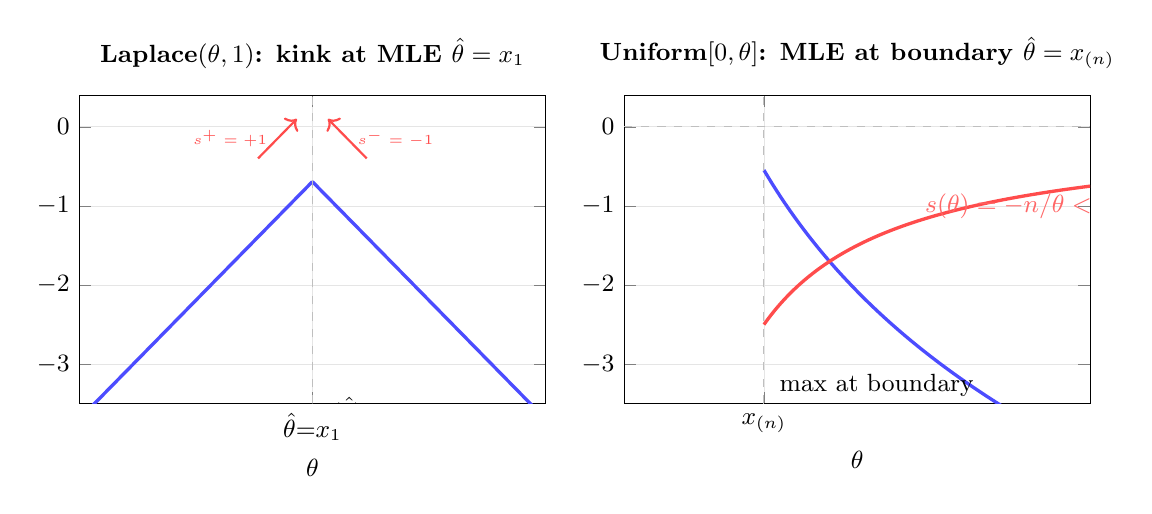
\begin{tikzpicture}
% Left: Laplace log-likelihood kink at MLE
\begin{axis}[
  name=left,
  width=7.5cm, height=5.5cm,
  xlabel={$\theta$},
  title={Laplace$(\theta,1)$: kink at MLE $\hat\theta=x_1$},
  xmin=-1.5, xmax=4.5, ymin=-3.5, ymax=0.4,
  domain=-1.5:4.5, samples=200,
  grid=both, grid style={line width=0.3pt,draw=gray!20},
  tick label style={font=\small},
  title style={font=\small\bfseries,align=center},
  label style={font=\small},
  xtick={1.5}, xticklabels={$\hat\theta{=}x_1$},
]
% ell(theta) = -|x1 - theta| + const; x1=1.5
\addplot[very thick,blue!70,domain=-1.5:1.5]{-(1.5-x) - 0.693};
\addplot[very thick,blue!70,domain=1.5:4.5]{-(x-1.5) - 0.693};
\addplot[dashed,gray!50] coordinates{(1.5,-3.5)(1.5,0.4)};
% left derivative arrow: slope=+1
\draw[->,red!70,thick] (axis cs:0.8,-0.4) -- (axis cs:1.3,0.1)
  node[midway,left,font=\tiny] {$s^+=+1$};
% right derivative arrow: slope=-1
\draw[->,red!70,thick] (axis cs:2.2,-0.4) -- (axis cs:1.7,0.1)
  node[midway,right,font=\tiny] {$s^-=-1$};
\node[font=\small,anchor=north] at (axis cs:1.5,-3.3)
  {$0\in\partial\ell(\hat\theta)$};
\end{axis}
% Right: Uniform[0,theta] — boundary max, score always negative
\begin{axis}[
  at={($(left.east)+(1cm,0)$)}, anchor=west,
  width=7.5cm, height=5.5cm,
  xlabel={$\theta$},
  title={Uniform$[0,\theta]$: MLE at boundary $\hat\theta=x_{(n)}$},
  xmin=0, xmax=4, ymin=-3.5, ymax=0.4,
  domain=1.2:4, samples=150,
  grid=both, grid style={line width=0.3pt,draw=gray!20},
  tick label style={font=\small},
  title style={font=\small\bfseries,align=center},
  label style={font=\small},
  xtick={1.2}, xticklabels={$x_{(n)}$},
]
% ell(theta) = -n*log(theta); n=3
\addplot[very thick,blue!70]{-3*ln(x)};
% score = -n/theta; n=3
\addplot[very thick,red!70]{-3/x};
\addplot[dashed,gray!50] coordinates{(1.2,-3.5)(1.2,0.4)};
\addplot[dashed,gray!50,domain=0:4,samples=2]{0};
\node[font=\small,red!60,anchor=west] at (axis cs:2.5,-1.0)
  {$s(\theta)=-n/\theta<0$};
\node[font=\small,anchor=north west] at (axis cs:1.25,-3.0)
  {max at boundary};
\end{axis}
\end{tikzpicture}
\caption{Non-smooth cases.
  Left: Laplace$(\theta,1)$ --- log-likelihood has a kink at the MLE;
  score does not exist there, but the MLE is well-defined.
  Left and right derivatives exist and have opposite signs:
  $0\in\partial\ell(\hat\theta)$ (subdifferential condition).
  Right: Uniform$[0,\theta]$ --- MLE at the boundary
  $\hat\theta=x_{(n)}$; score $s(\theta)=-n/\theta<0$ everywhere on
  the interior, so no stationary point exists.}
\label{fig:nonsmooth}
\end{figure}

\paragraph{Case 1: non-differentiable likelihood (Laplace).}
For $p(x\mid\theta)=\tfrac{1}{2}e^{-|x-\theta|}$, the log-likelihood
$\ell(\theta)=-|x_1-\theta|+\text{const}$ has a kink at $\theta=x_1$.
The MLE is the argmax, but characterised by the subdifferential
condition $0\in\partial\ell(\hat\theta)$, not by $s(\hat\theta)=0$.

\paragraph{Case 2: boundary maximum (Uniform).}
For $X_i\sim\mathrm{Uniform}[0,\theta]$, $\ell(\theta)=-n\log\theta$
for $\theta\geq x_{(n)}$.  The score $s(\theta)=-n/\theta<0$ is
strictly negative on the interior: the log-likelihood is monotone
decreasing, so the maximum is at the boundary $\hat\theta=x_{(n)}$.
No stationarity condition applies.

\begin{remark}
The LM test theory assumes the regular smooth interior case.
For non-smooth likelihoods, subgradient methods or boundary
corrections are required.
\end{remark}

%--------------------------------------------------------------------

%====================================================================

\end{document}
